%
%\newcommand{\CLASSINPUTinnersidemargin}{13mm}
%\newcommand{\CLASSINPUToutersidemargin}{10mm}
\documentclass[10pt,journal,a4paper,onecolumn]{IEEEtran}
%\documentclass[journal]{IEEEtran}

%\usepackage[norsk]{babel}
\usepackage[latin1]{inputenc}
%\usepackage[T1]{fontenc}
% correct bad hyphenation here
\hyphenation{op-tical net-works semi-conduc-tor}

% added by Erlend
\usepackage{amsmath}%
\usepackage{amsfonts}%
\usepackage{amssymb}%
\usepackage{amsthm}%
%\usepackage{mwe}
\usepackage[pdftex]{graphicx}
%\usepackage{graucx}
\usepackage{epsfig} 
%\usepackage{mwe}    % loads �blindtext� and �graphicx�
%\usepackage{subfig}
%\usepackage{caption}
\usepackage{subfloat}
%\usepackage{subcaption}
%\usepackage{subfigure} 
\usepackage{url}
\usepackage{epstopdf}
%\captionsetup[subfig]{margin=2mm,format=hang}
%\usepackage{subcaption}
\usepackage{float}
%\usepackage{algorithm} 
%\usepackage{algorithmic} 
\usepackage{setspace}
%\usepackage[utf8]{inputenc}
\usepackage{overpic}
\usepackage{color}
\usepackage{enumerate}
\usepackage{comment}
\usepackage{lipsum,amsmath,multicol}

% added by constantin
\usepackage{siunitx}%
\usepackage{booktabs}%
% \usepackage{multicol}%
\usepackage{multirow}

% for subfig
\usepackage{subfig}
%\usepackage[caption = false]{subfig}
%\usepackage[demo]{graphicx}

\setstretch{1.3}
\setlength{\columnsep}{1.0cm}

\newtheorem{theorem}{Theorem}[section]
\newtheorem{lemma}[theorem]{Lemma}
\newtheorem{requirement}[theorem]{Requirement}

%\setlength{\topmargin}{0.0cm}
%\setlength{\textheight}{21.5cm}
%\setlength{\oddsidemargin}{0cm} 
%\setlength{\textwidth}{15.5cm}
%\setlength{\columnsep}{0.6cm}


\newcommand{\qi}{q_{\mathrm{in}}}
\newcommand{\Qso}{Q_{\mathrm{so}}}
\newcommand{\tQso}{\tilde{Q}_{\mathrm{so}}}
\newcommand{\Qsi}{Q_{\mathrm{si}}}
\newcommand{\tQsi}{\tilde{Q}_{\mathrm{si}}}
\newcommand{\q}{\vec{q}}
\newcommand{\xso}{x_\mathrm{so}}
\newcommand{\xsi}{x_\mathrm{si}}
\newcommand{\ce}{c^\epsilon}
\newcommand{\tphi}{\tilde{\phi}}
\newcommand{\R}{\mathbb{R}}
\newcommand{\CHalert}[1]{\textcolor{red}{CH: #1}}
\newcommand*\diff{\mathop{}\!\mathrm{d}}

\DeclareSIQualifier{\hundret}{100}


\begin{document}

\title{A validation of the classical one-compartment model for perfusion}
\author{Constantin Heck, \and Erlend Hodneland, \and Erik A. Hanson, \and Arvid Lundervold, \and Jan Modersitzki, \and Alexandre Malyshev
\thanks{Erlend Hodneland is with Clinical Department 1, University of Bergen, Norway.}
(Random order)
\thanks{}

}


%\date{February 24, 2002}
\maketitle



% The paper headers
\markboth{Image processing,~Vol.~x, No.~x, January~20xx}%
{Shell \MakeLowercase{\textit{et al.}}: A validation study of the classical theory for one-compartment indicator dilution.}



% make the title area
\maketitle



% Note that keywords are not normally used for peerreview papers.
\begin{IEEEkeywords}
Porous media flow, indicator, brain DCE-MRI
\end{IEEEkeywords}





% For peerreview papers, this IEEEtran command inserts a page break and
% creates the second title. It will be ignored for other modes.
\IEEEpeerreviewmaketitle

\begin{abstract}
\end{abstract}
\section{Mathematical theory}

\subsection{A synthetic one-compartment single-phase flow model}

A synthetic one-compartment (1C) model of the plasma flow within a porous organ can be developed from the principle of mass balance and Darcys law. Denote the porosity $\phi = \phi(x,t)$ with units $ m^3/m^3$ as the relative quantity describing the fluid volume within a control volume $\Omega_i$ divided by the total volume of $\Omega_i$. Within the classical theory of compartment modelling for human organs the porosity is better known as the cerebral blood volume (CBV).  The fluid density has units $(kg/m^3)$ and is denoted by $\rho = \rho(x,t)$. We apply the geomechanical understanding of flux as a surface flux $q = q(x,t)$ with units $(m^3/s/m^2)$. The surface flux is a vector field describing the volume of fluid per unit time flowing across a sliced unit area of the sample. The continuity equation reflecting conservation of mass within the fluid states
\begin{equation}
\frac{\partial (\phi \rho)}{\partial t} + \nabla \cdot (\rho q) = \tilde{Q}
\label{eq:syntcont}
\end{equation}
where $\tilde{Q} = \tilde{Q}(x,t)$ is a source or sink of fluid mass with units $kg/s/m^3$. For the current task we want to model the perfusion of blood in the brain and we consider it a stationary process. This assumption is only partly true due to factors like external stress which can influence the flow pattern. However, it is still a reasonable and common approximation. By these simplifications the porosity, fluid density and flux are only functions of space, $\phi = \phi(x), \rho = \rho(x), q = q(x)$. Furthermore we assume that the fluid density $\rho$ is constant in space, which is satisfied within all practical means for water within the human body.  The continuity equation (\ref{eq:syntcont}) then becomes
\begin{equation}
\nabla \cdot q = \frac{\tilde{Q}}{\rho}.
\label{eq:syntcontsimp}
\end{equation}
In order to scale away the density $\rho$ we define another source term $Q$ with units $m^3/s/m^3$ having the relation $\tilde{Q} = Q\rho$, thus transforming (\ref{eq:syntcontsimp}) into
\begin{equation}
\nabla \cdot q = Q.
\label{eq:syntcontsimp2}
\end{equation}
The right hand side is only non-zero within the source or the sink. Elsewhere, (\ref{eq:syntcontsimp2}) is concurrent with the incompressibility condition of divergence free flow.

Low velocity fluid flow in porous media is described by Darcys law
\begin{equation}
q = -\frac{K}{\mu}\Big ( \nabla p + \rho g  \nabla z\Big )
\label{eq:syntdarcy}
\end{equation}
where $g$ is the gravitational acceleration, $K$ is the permeability tensor in units $m^2$, $z$ is the spatial position along the gravitational field and $\mu = \mu(x)$ is the viscosity of the fluid with units $Pa \cdot s$.
For the current project the flow is taking place perpendicular to the gravitational field and the gravitational term can thereby be discarded, such that a simplified version of Darcys law becomes
\begin{equation}
q = -\frac{K}{\mu} \nabla p.
\label{eq:syntdarcysimp}
\end{equation}
Moreover, assuming a hermitian and positive definite permeability tensor $K$, and combining (\ref{eq:syntcontsimp2}) and (\ref{eq:syntdarcysimp}) results in the elliptical operator
\begin{equation}
\nabla \cdot \Big ( -\frac{K}{\mu} \nabla p\Big ) = Q
\label{eq:flowmodel}
\end{equation}
for the scalar pressure field $p$.
Denote the boundary of $\Omega$ as $\partial \Omega$, with an outward normal vector $n(x)$. We impose Neuman boundary conditions of no pressure gradient across the boundary, thus $\nabla p \cdot n = 0$ on $\partial \Omega$. This conditions is equivalent to no flow across the boundary. Equation (\ref{eq:flowmodel}) in combination with Neuman boundary conditions $\nabla p \cdot n = 0$ on $\partial \Omega$ is the flow model we apply to create the synthetic brain template.
The flux field can be computed according to (\ref{eq:syntdarcy}) from the obtained pressure map. An example of pressure and flux fields is shown in Fig. \ref{fig:flowsyntresults} (a) - (c).


\subsection{The forward problem for indicator dilution}

In this section we add a tracer to the flow entering via the source, where the aim is to describe how the tracer is carried along within the flow. The concentration map resulting from the simulation is later used as a model for observed concentrations as they could appear from a MR scan. We will apply this concentration for the inverse problem of determining the perfusion and porosity. By comparing the inversely reconstructed perfusion with the known perfusion we can validate the classical models for CBV and CBF. 


Denote the space and time depending tracer concentration with respect to the fluid space as $c(x,t)$, with units $Mol/m^3$. Also, denote the tracer concentration with respect to a control volume as $C(x,t)$, also with units $Mol/m^3$. Thus, for $c(x,t)$ the normalizing volume refers to the fluid volume and for $C(x,t)$ the normalization refers to the control volume. The units $Mol/m^3$ are applied instead of the classical units $mMol/L$ in order to be compatible with $Q(x)$ having units $m^3/s/m^3$. 

The porosity is from definition $\phi_i=v_i/V_i$ for a plasma volume $v_i$ within a control region $\Omega_i$ having a total volume of $V_i$. Letting $|\Omega_i| \rightarrow 0$ leads to the continuos porosity field $\phi$. Denote the number of tracer molecules within a control roi as $n_i$. From the definition of $c$ and $C$, we obtain the relation $n_i = cv_i = CV_i$. Combining this with $\phi_i = v_i/V_i$ leads to $C_i = c_i\phi_i$, approaching the continuous formulation $C = c\phi$ as $|\Omega_i|\rightarrow 0$. 

The rate of change of tracer molecules within a geometric control volume $\Omega_i$ can he phrased as
\begin{equation}
	\frac{\partial }{\partial t}\int_{\Omega_i}Cdx = \int_{\Omega_i}\frac{\partial }{\partial t}(\phi c)dx.
	\label{eq:dmdt}
\end{equation}
By discarding any dissipative diffusion process, the change in tracer mass within $\Omega_i$ occurs only from advective flow and source/sink terms as
\begin{equation}
	-\int_{ \Gamma_i}c(q \cdot \nu)ds + \int_{\Omega_i}c_{so}Q_{so}dx + \int_{\Omega_i}cQ_{si}dx
	\label{eq:surfflux}
\end{equation}
where $Q_{so}(x)\geq 0$ $[m^3/s/m^3]$ is the source term and $Q_{si}(x)\leq 0$ $[m^3/s/m^3]$ is the sink term which both are zero everywhere except from in the respective source/sink locations. Note that $\int_\Omega Q_{so}dx = -\int_\Omega Q_{si}dx$, in line with incompressible flow. The point wise relation between $Q$, $Q_{so}$ and $Q_{si}$ is $Q = Q_{so} + Q_{si}$. From preservation of the tracer mass, equations (\ref{eq:dmdt}) and (\ref{eq:surfflux}) must balance such that
\begin{equation}
	\int_{\Omega_i}\frac{\partial }{\partial t}(\phi c)dx + \int_{ \Gamma_i}c(q \cdot \nu)ds = \int_{\Omega_i}c_{so}Q_{so}dx + \int_{\Omega_i}cQ_{si}dx.
	\label{eq:conteq}
\end{equation}
Assuming a stationary porosity $\phi$, this can be rewritten as 
\begin{equation}
	\int_{\Omega_i}\phi\frac{\partial c}{\partial t}dx + \int_{ \Gamma_i}c(q \cdot \nu)ds = \int_{\Omega_i}c_{so}Q_{so}dx + \int_{\Omega_i}cQ_{si}dx.
	\label{eq:conteq2}
\end{equation}
Upon application of the divergence theorem, Eq. (\ref{eq:conteq2}) is consistent with the continuity equation on local form
\begin{equation}
	\phi \frac{\partial c}{\partial t} + \nabla \cdot (cq) = c_{so}Q_{so} + cQ_{si},
	\label{eq:conteqlocal}
\end{equation}
a quasi-linear transport equation in $c(x,t)$. 
\\
BEGIN COMMENT FROM HERE, INTERMEDIATE STEPS, ONLY FOR CLARIFICATION UNTIL SUBMISSION
\\
This is equivalent to
\begin{equation}
	\phi \frac{\partial c}{\partial t} + c \nabla \cdot q  + q \cdot \nabla c = c_{so}Q_{so} + cQ_{si},
	\label{eq:conteqlocaltemp}
\end{equation}
This is equivalent to
\begin{equation}
	\phi \frac{\partial c}{\partial t} + cQ  + q \cdot  \nabla c = c_{so}Q_{so} + cQ_{si}
	\label{eq:conteqlocaltemp}
\end{equation}
This is equivalent to
\begin{equation}
	\phi \frac{\partial c}{\partial t} + cQ_{so} + c Q_{si}  + q \cdot  \nabla c = c_{so}Q_{so} + cQ_{si}
	\label{eq:conteqlocaltemp}
\end{equation}
This is equivalent to
\begin{equation}
	\phi \frac{\partial c}{\partial t} + cQ_{so}  + q \cdot  \nabla c = c_{so}Q_{so}
	\label{eq:conteqlocaltemp}
\end{equation}
This is equivalent to
\begin{equation}
	\phi \frac{\partial c}{\partial t} + q \cdot  \nabla c = c_{so}Q_{so} -  cQ_{so} 
	\label{eq:conteqlocaltemp}
\end{equation}
This is equivalent to
\begin{equation}
	\phi \frac{\partial c}{\partial t} + q \cdot  \nabla c = (c_{so} -  c)Q_{so}
	\label{eq:conteqlocaltemp}
\end{equation}
END COMMENT FROM HERE
\\
The input tracer concentration $c_{so}$ is assumed known at all time points as well as the source and sink terms $Q_{so}$ and $Q_{si}$. Inserting (\ref{eq:syntcontsimp2}), applying $Q = Q_{si} + Q_{so}$ and dividing by the non-zero porostiy $\phi$ leads to
\begin{equation}
	\phi \frac{\partial c}{\partial t} + q\cdot\nabla c = (c_{so}-c)Q_{so}.
	\label{eq:conteqlocal2}
\end{equation}
%Given the source/sink field $Q(x)$ we state the continuity equation for the tracer molecules
%\begin{equation}
%\frac{\partial (\phi c)}{\partial t} + \nabla \cdot (cq) = cQ.
%\label{eq:syntconttracer}
%\end{equation}
%Dealing with Gadolinium based tracers, we can safely assume that the tracer is not created or destroyed within the domain and the entire source/sink of tracer is therefore via the fluid source/sink $Q$. Furthermore, we assume a homogeneous mixing of tracer within the incoming fluid. Adding a volume integral over the control region $\Omega_i$ to each side of (\ref{eq:syntconttracer}), as well as applying the divergence theorem leads to
%\begin{equation}
%\int_{\Omega_i} \phi\frac{\partial c}{\partial t}dx =  - \int_{\Gamma_i}c (q \cdot \nu)ds + \int_{\Omega_i}cQdx
%\label{eq:syntconttracer1}
%\end{equation}
%for a positive outward pointing normal vector $\nu$, and where we also used the stationarity assumption of $\phi$.
%Only the normal flux component $q_n$ contributes to tracer transport across the faces of the control volume, and therefore
%\begin{equation}
%\int_{\Omega_i} \phi\frac{\partial c}{\partial t}dx =  - \int_{\Gamma_i}c q_nds + \int_{\Omega_i}cQdx.
%\label{eq:syntconttracer2}
%\end{equation}
%Using a Cartesian grid, the normal component $q_n$ will be aligned with the main coordinate directions. Equations (\ref{eq:flowmodel}) and (\ref{eq:syntconttracer2}) together constitute the synthetic model for flow and indicator dilution. 
We refer to (\ref{eq:conteq2}) and (\ref{eq:conteqlocal2}) as the \textit{simulated flow model (SF model)}. Equation (\ref{eq:conteq2}) is implemented under the assumption of (\ref{eq:syntcontsimp2}), which the obtained flux $q$ is fulfilling.
Equation (\ref{eq:conteq2}) is used for numerical simulations and (\ref{eq:conteqlocal2}) is only used for analytical considerations.
%In this respect, note that it can be written in the standard form of a quasi-linear transport equation as
%\begin{equation}
%	v \cdot D c = f(x,c)
%	\label{eq:conteqlocal3}
%\end{equation}
%for $v = (q,\phi)$, the spatio-temporal gradient $D = (\nabla,\partial/\partial t)$ and the right hand side $f = (c_{so}-c)Q_{so}$.

\subsection{Conversion of flux into perfusion}\label{subsec:FluxToPerfusion}
The SFM uniquely determines the flux field $q(x)$. However, it is not obvious how to transform a flux field into a scalar perfusion field $P(x)$, a widely used parameter in the classical field of compartment modelling. There are at least two obvious differences between $q$ and $P$. First, the flux is a vector field and the perfusion is a scalar field. Second, the flux relates to a surface area and the perfusion relates to a volume. Thus, these to quantities are strictly, mathematically different but still conceptually related. In the following we describe a method for converting flux into perfusion.

The classical understanding of perfusion is the amount of blood feeding a tissue volume per unit time. Thus, the perfusion $P$ has the units $m^3/s/m^3$. It is common to scale this quantity to normalized perfusion $P_n(x)$ with units $ml/min/100ml$. 
One approach for converting flux into perfusion could be to estimate the perfusion as the total inflow (or outflow) of fluid (e.g. arterial blood) into a control region per unit time, and then normalizing with the control region volume. This is only a valid approach if every control region is separated from other control regions, and not feeding each other. Thus, this approach is valid for an entire organ being the control region. Such understanding is in line with the understanding of classical compartment models for perfusion where each voxel has its own source of feeding arterial blood, independent of the neighbour voxels. Clearly, this is a simplification since voxels will be fed by their neighbours. In our synthetic flow model SFM as well as in normal tissue this assumption is violated since the voxels are feeding their neighbour voxels with arterial blood. Simply summing the total inflow into a voxel and dividing by the voxel volume will strongly over-estimate the perfusion since we would divide by the wrong normalization volume. The problematic issue is that the incoming blood is feeding more voxels than the current voxel. This phenomenon is demonstrated in Fig. \ref{fig:perfusion-problem} where the volume on the left has the true perfusion value of $P_1 = F_0/(2V)$ for an incoming flow $F_0$ $[m^3/s]$ and distribution volume $2V$ $[m^3]$. However, for another discretization as shown in the middle, the perfusion within each of these sub-volumes becomes $P_2 = F_0/V = 2P_1$. Taking the average across both sub-volumes, it is clear that the perfusion is over-estimated with a factor of two. A discretization dependent perfusion value is not desirable, and the perfusion estimate of $P_2$ is clearly wrong. 


\begin{figure}[H]
    \centering
    \begin{overpic}[scale=0.5]{figs/perfusion-problem.eps}
    	\put(11,67){\color{black}$F_0$}
	\put(49,67){\color{black}$F_0$}
	\put(85.2,66){\color{black}$\Delta F_0$}
	\put(13,33){\color{black}$2V$}	
	\put(50,20){\color{black}$V$}	
	\put(50,45){\color{black}$V$}	
	\put(91,42){\color{black}$\Delta V$}	
	\end{overpic}
    \caption{Perfusion within a small volume. Left: A compartment with volume $2V$ is exposed to a flow $F_0$ $ [m^3/s]$ of fluid. From definition, the overall perfusion within this object becomes $P_1 = F_0/(2V)$ $m^3/s/m^2$. Right: The volume is divided into two smaller compartment (e.g. voxels), and the perfusion for each of the compartments becomes $P_2 = F_0/V = 2P_1$. This discrepancy between the two discretisation regimes occurs because the flow is counted twice as it is feeded from one voxel to the other. Right: As a solution to the described problem we pick out a true distribution volume $\Delta V$ (area in this 2D sketch), which is a small area around a given streamline along the centre line of the grey area. This is the true distribution volume (area) which is feeded with arterial blood from the incoming fractional flow $\Delta F_0$. The correct perfusion within $\Delta V$ is therefore $\Delta F_0/dV$. The entire compartment can further be divided into infinitesimal distribution volumes, thus providing voxelwise perfusion values.}
    \label{fig:perfusion-problem}
\end{figure}

The reason for this discrepancy is that for $P_2$ the perfusion has been counted twice since we are dividing by the wrong distribution volume. Instead, we need to consider to the classical definition of perfusion. The concept of perfusion has a very precise meaning, as the amount of arterial blood per time unit delivered to a capillary bed in a biological tissue, and then scaled by the feeded tissue volume. Therefore, we must divide the incoming flow by the total distribution volume that is covered by the fluid streamlines. This formulation coincides with the classical understanding of perfusion, and the correct distribution volume will rather be the volume that the fluid particles within an infinitesimal cross-sectional area around the streamlines are covering. Assuming laminar flow, the streamlines are not crossing each other and we can with this formulation correctly estimate the true distribution volume that is fed by a given arterial blood flow.

Formally, the direction of the streamline vector field is identical to the flux vector field mediating the flow. Pick an area $S$ around a streamline, where $S$ is formed as a disc with area $A = \pi r^2$ and infinitesimal area $dA = 2\pi r dr$. The flow in $m^3/s$ passing the cross-sectional area $S$ becomes
\begin{equation}
	F_S = \int_S(q \cdot n)dA = \int_0^R(q \cdot n)2\pi r dr
\end{equation}
for a unit vector $n$ pointing along with the flow, and where $R$ is the radius of $S$. Since the flux is carrying the flow, $n = q/|q|$ and the flow $F_S$ across $S$ becomes
\begin{equation}
	F_S = 2\pi\int_0^R |q| r dr.
\end{equation}
The total distribution volume that the flow is passing through can be estimated as
\begin{equation}
	V_S = \int_0^L\int_SdAdl
\end{equation}
which is equivalent to
\begin{equation}
	V_S = 2\pi\int_0^L\int_0^Rrdrdl,
\end{equation}
where $L$ is the upper line integration limit of a streamline from inlet to outlet. We can now formalize a precise perfusion measure in agreement with the physiological concept of perfusion as
\begin{equation}
P = \lim_{R \rightarrow 0}\frac{F_S}{V_S} = \lim_{R \rightarrow 0}\frac{\int_0^R|q|rdr}{\int_0^L\int_0^Rrdrdl}.
\end{equation}
Using L'Hopitals rule we reach a locally well defined perfusion measure
\begin{equation}
P(x) = \frac{|q(x)|}{|\mathbb{C}|(x)|}
\label{eq:flux2perf}
\end{equation}
where $||\mathbb{C}(x)| = \int_0^Ldl$ is the length of the streamline passing through the point $x$. This is an explicit formula for converting flux into perfusion and is later used for evaluation of the classical model for perfusion. With the model in (\ref{eq:flux2perf}) we realize that every point along a streamline will have the same value of perfusion. This is reasonable since these voxels are fed by the same flow. 


\subsection{Estimating the porosity}
The principle of mass balance of fluid and tracer particles is described by Eq.  (\ref{eq:syntcontsimp2}) and (\ref{eq:conteqlocal}). For locations where the source and sink is zero, $Q_{so}(x) = 0$ and $Q_{si}(x) = 0$, and (\ref{eq:conteqlocal}) becomes
\begin{equation}
\phi\frac{\partial c}{\partial t}  = - q \cdot \nabla c.
\label{eq:1cmodel}
\end{equation}
Integrating from $t_0$ to $t_1$ results in the model
\begin{equation}
\phi [c(x,t_1) - c(x,t_0)]  = - \int_{t_0}^{t_1}q \cdot  \nabla c dt.
\label{eq:1cmodel1}
\end{equation}
Inserting $t_0 = - \infty$ to $t_1 = \infty$ and boundary conditions $c(x,-\infty) = c(x,\infty) = 0$ leads to
\begin{equation}
q \cdot \nabla  \int_{-\infty}^{\infty} c(x,t)dt = 0
\label{eq:streamlinezero}
\end{equation}
since $q$ is independent of time. Equation (\ref{eq:streamlinezero}) states that $\int_{-\infty}^{\infty} c(x,t)dt$ is constant along the streamlines of the fluid flow.
Thus, we can choose any voxel in the downstream from the arterial input such that
\begin{equation}
\int_{-\infty}^{\infty} c(a,t)dt = \int_{-\infty}^{\infty} c(x,t)dt
\end{equation}
where $c(a,t)$ is the tracer concentration of the arterial input, and assuming the region of interest (ROI) for the arterial input is a infinitesimal small point in space for the spatial position $x = a$. Using $C = \phi c$ and assuming the porosity of the arterial inlet is known (and typically close to one), here denoted by $\phi_a$, we have an analytical expression for the porosity at any position $x$,
\begin{equation}
\phi(x) = \phi_a \frac{ \int_{-\infty}^{\infty} C(x,t)dt }{ \int_{-\infty}^{\infty} C(a,t)dt}.
\label{eq:phi}
\end{equation}
Note the boundary conditions that were used to arrive at this expression. Practially, $c(x,t \rightarrow \infty)$ will never go to zero and one possible solution to this problem is to fit a gamma curve to the data, approaching zero as $t \rightarrow \infty$.
The expression reached in (\ref{eq:phi}) coincides with the classical formula for CBV and is hereby analytically proven for a one-compartment model.



\subsection{Classical model for perfusion}

Denote as $N$ the number of tracer molecules within a given compartment. Conservation of tracer molecules within the compartment leads to the differential equation
\begin{equation}
\frac{dN}{dt} = N_{a} - N_{out}
\label{eq:dndt}
\end{equation}
where $N_{a}$ and $N_{out}$ are the number of tracer molecules entering or leaving the control region per unit time. Equation (\ref{eq:dndt}) can be written as
\begin{equation}
\frac{dN}{dt} = \tilde{P}_{a}c_{a}(t) - \tilde{P}_{out}c_{out}(t)
\label{eq:dndt2}
\end{equation}
where $\tilde{P}_{a},\tilde{P}_{out}$ are the non-normalized perfusion $[mm^3/s]$ entering or leaving the system, respectively, and where $c_a(t)$ is the tracer concentration at the inlet.
Due to the incompressibility condition, $\tilde{P}_{a} = \tilde{P}_{out} = \tilde{P}$, and assuming a well-mixed fluid compartment leads to
\begin{equation}
\frac{dN}{dt} = \tilde{P}(c_{a}(t) - c(t))
\end{equation}
where $c(t)$ is the tracer concentration within the compartment.
Dividing by the control volume $V$ we get
\begin{equation}
\frac{dC}{dt} = P(c_{a}(t) - c(t)).
\end{equation}
for $C = N/V$ and $P = \tilde{P}/V$, noting that $P$ is the fluid volume flow per unit time per unit tissue volume $[mm^3/s/mm^3]$, known as the perfusion or $CBF$ when applied within the cortex of the brain. The subscript refers to the classical formulation of perfusion.
This ODE can be rephrased as
\begin{equation}
\frac{dc}{dt} -\frac{P}{\phi}c(t)  = \frac{P}{\phi}c_{a}(t).
\end{equation}
For a stationary perfusion $P$ this equation has the general solution
\begin{equation}
c(t) = \frac{P}{\phi} \int_{t_0}^{t}e^{-\frac{P}{\phi}(t-s)}c_a(s)ds + D e^{-\frac{P}{\phi}(t)}
\end{equation}
Assuming no tracer at $t = t_0$ and setting $t_0 = 0$ leads to the requirement $D = 0$, and the solution becomes
\begin{equation}
c(t) = \frac{P}{\phi} \int_{0}^{t}e^{-\frac{t-s}{T}}c_a(s)ds
\end{equation}
for the mean transit time $T \equiv \phi/P $. Incorporating $C = c\phi$ leads to
\begin{equation}
C(t) = P \int_{0}^{t}e^{-\frac{t-s}{T}}c_a(s)ds.
\label{eq:Cconv}
\end{equation}
Deconvolution of (\ref{eq:Cconv}) is the classical model for estimating the perfusion $P$ with a known residue function $R(t) = e^{-t/T}$.
Denote the impulse response function $I(t) = P R(t)$. Equation (\ref{eq:Cconv}) can then equivalently be written as a convolution
\begin{equation}
C(t) = I(t) * c_a(t)
\label{eq:Cconv1}
\end{equation}
provided $c_a(t)$ is zero for $t < 0$. 

Applying the forward model in (\ref{eq:Cconv1}) for a known perfusion $P$ leads to a simulated flow model based on convolution, in accordance with the classical theory. We refer to this model as the \textit{simulated convolution model (SC model)}. We have now defined two competing models for indicator dilution, the SF model and the SC model. This was done in order to be able to discover any discrepancies from the true perfusion field and relate them to shortcomings in the model itself or to instability of the numerical deconvolution. 

\subsection{Relating the simulated flow (SF) model with the classical model for perfusion}
Consider the solute transport equation (\ref{eq:conteqlocal}), and rewrite it as
\begin{equation}
	\frac{\partial c}{\partial t} + \frac{q}{\phi} \cdot \nabla c = \frac{(c_{so}-c)Q_{so}}{\phi }.
	\label{eq:conteqlocal3}
\end{equation}
We follow the method of characteristics and first convert from Eulerican coordinates $(x,t)$ to Lagrangian coordinates $(x_0,t_0)$, the beginning of a streamline. Here $(x_0,t_0)$ is fixed the parameterizatiton parameter for the streamline emerging at $(x_0,t_0)$ will be denoted by $s$. 
Substituting $x = x(s)$, $t=t(s)$ and denoting $c(s):=c(x(s),t(s))$, $\Qso(s):=Q_{so}(x(s))$, $\phi(s):=\phi(x(s))$ and $c_a(s):=c_a(t(s))$  yields the following system of ODEs [cite Evans]:
\begin{subequations}
	\label{eq:ODEs}
	\begin{alignat}{2}
		c'(s) + \frac{\Qso(s)}{\phi(s)}C(s) &= \frac{c_a(s)\Qso(s)}{\phi(s)}, & \quad c(0) &= 0 \label{eq:ODEC} \\
		x'(s) &= \frac{q(s)}{\phi(s)}, &x(0) &= x_0 \label{eq:ODEx}\\
		t'(s) &= \phi(s),     &t(0) &= t_0, \label{eq:ODEt}
	\end{alignat}
\end{subequations}
Here $x_0$ denotes the starting-point (in space) of the streamline and $t_0$ denotes the starting-timepoint of the streamline. $c(s)$ hence can be regarded the concentration curve of a particle which originated at $(x_0,t_0)$ and $(x(s),t(s))$ is the wavefront at artificial timepoint $s$. For a visualization see Fig. \ref{fig:Streamlines}.
\begin{figure}[H]
	\begin{tabular}{c p{3cm}}
		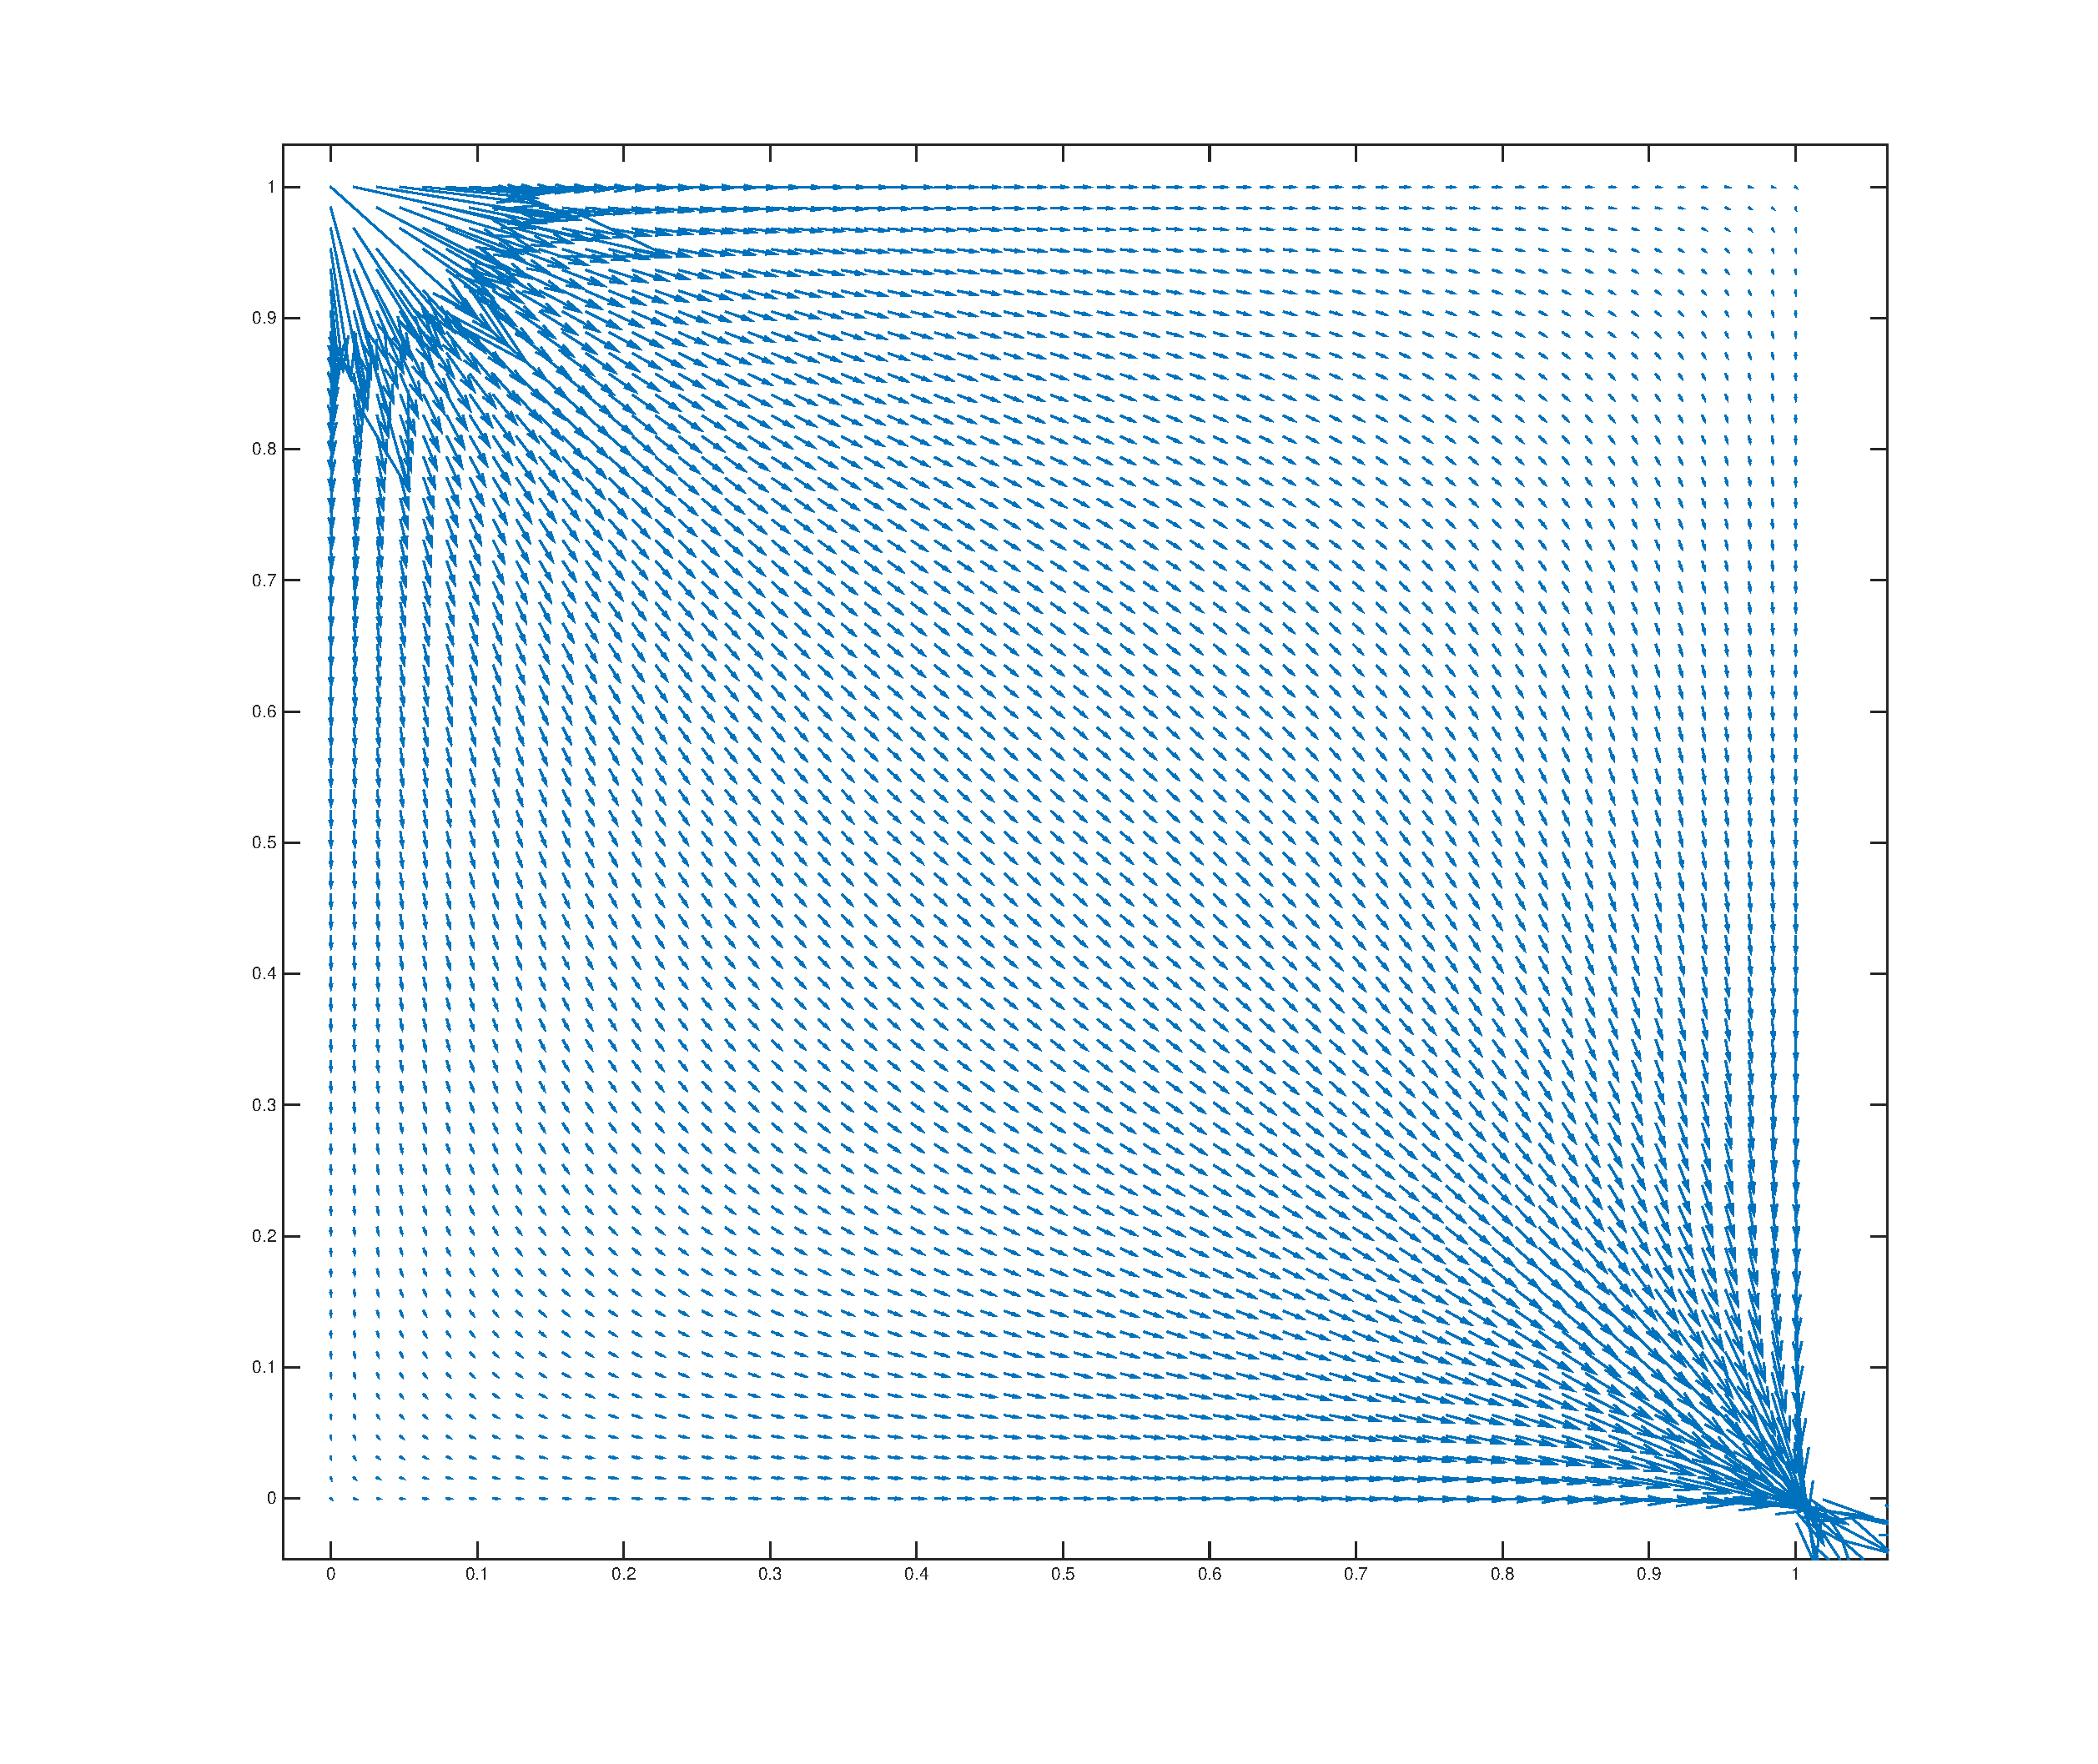
\includegraphics[width=10cm]{./figs/vectorField.eps} &\vspace{-5cm}\parbox{3cm}{Flow field $q(x)$}\\
		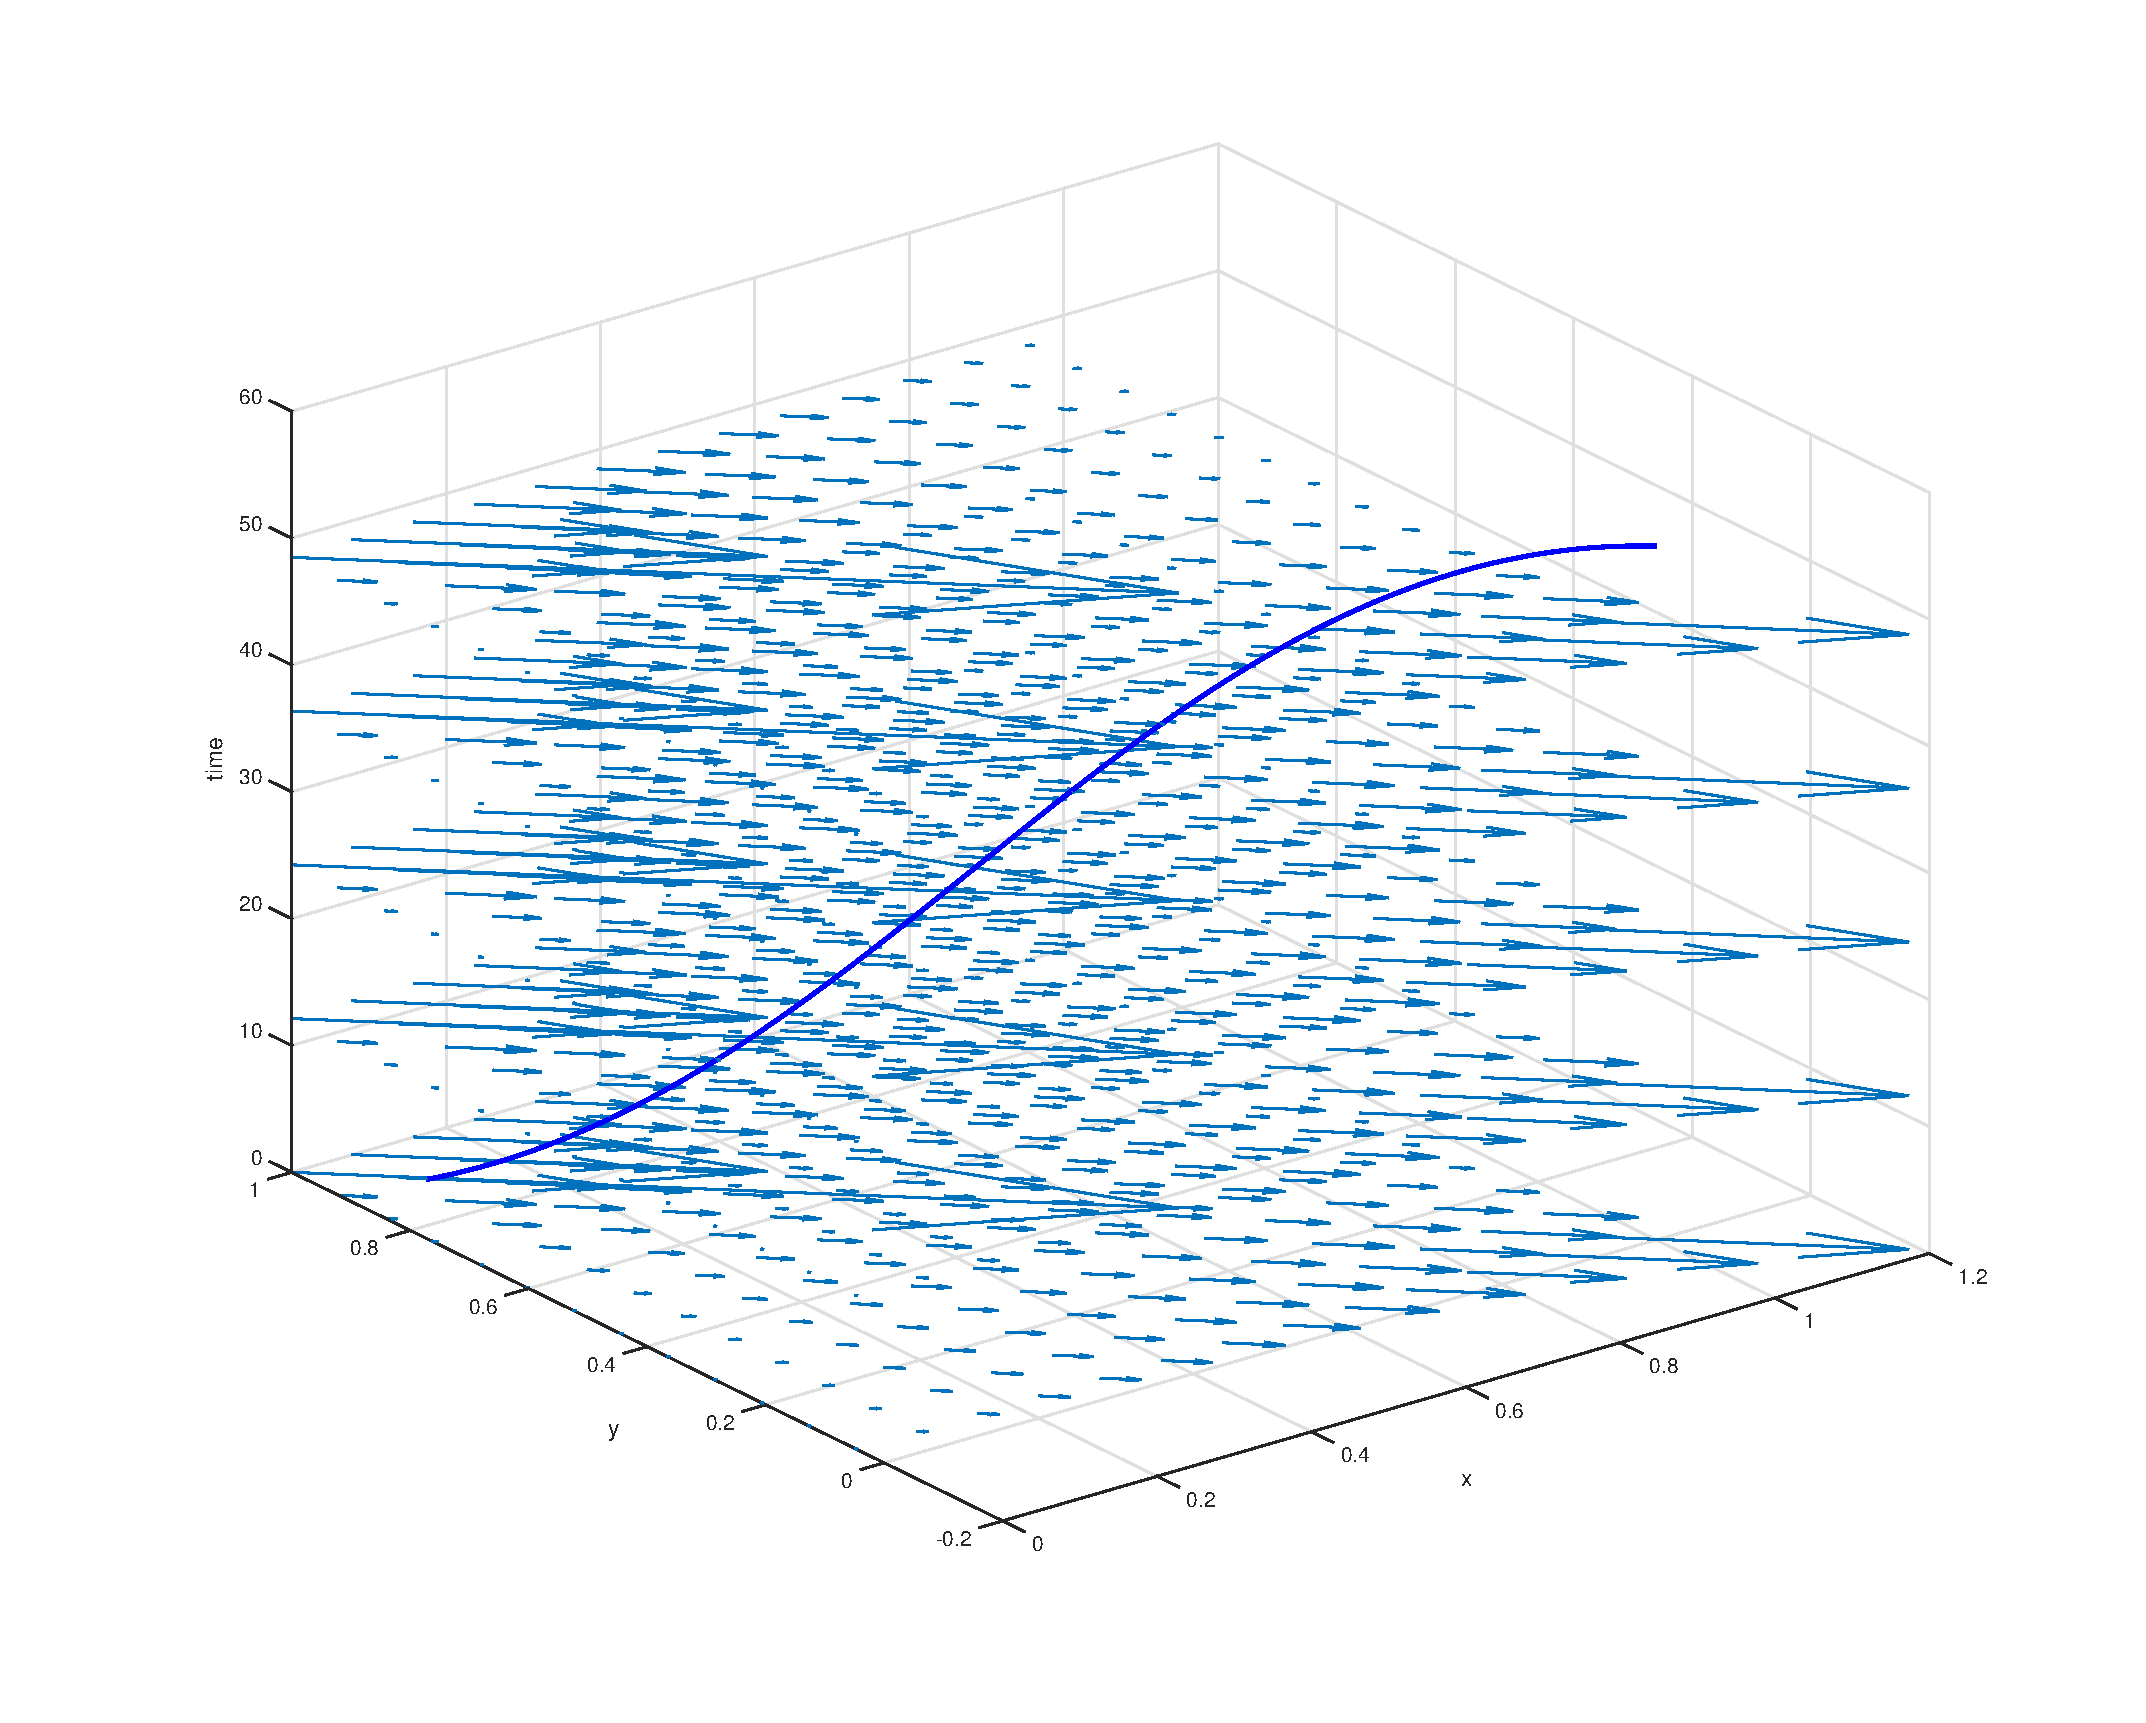
\includegraphics[width=10cm]{./figs/singleStreamline.eps} &\vspace{-5cm}\parbox{3cm}{A single streamline emerging at point $x_0 = (0.1,0.9)$} \\
		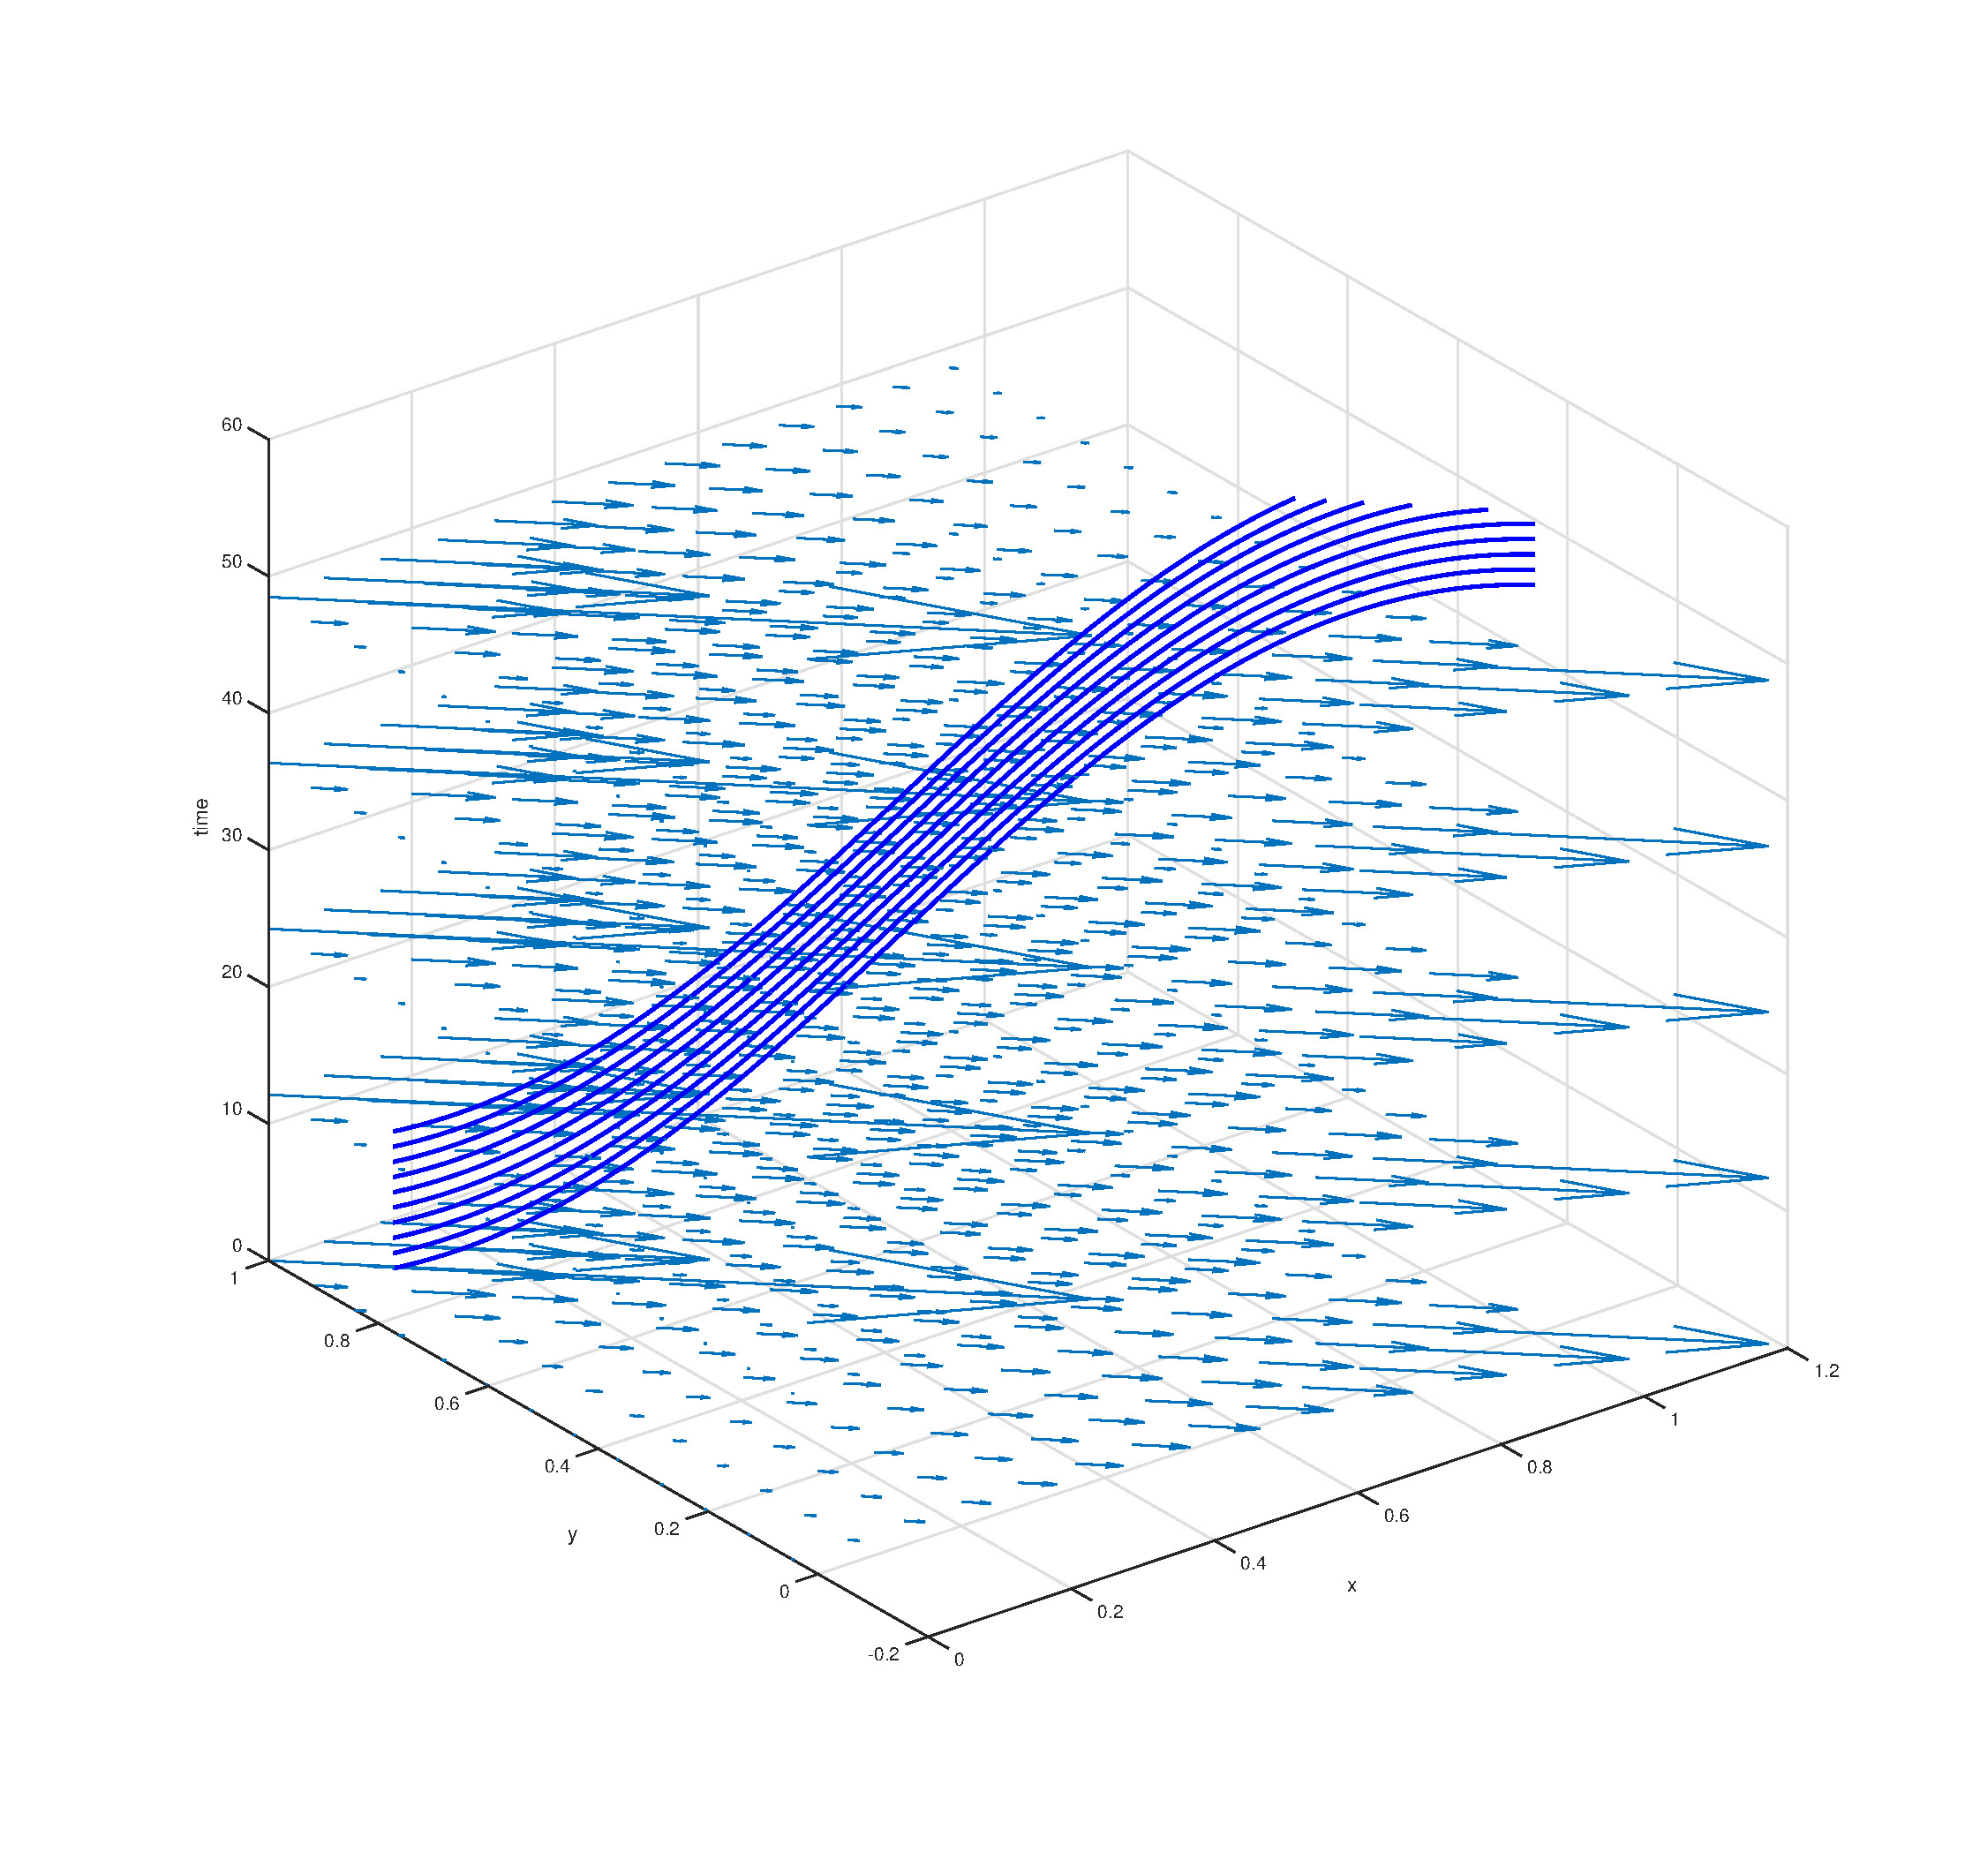
\includegraphics[width=10cm]{./figs/multipleStreamlines.eps} &\vspace{-5cm}\parbox{3cm}{Multiple Streamlines emerging at point $x_0=(0.1,0.3)$ at different timepoints.}
	\end{tabular}
	\caption{Flow-Field and Streamlines}
	\label{fig:Streamlines}
\end{figure}
Let the source term be non-zero within the ball $B_\epsilon$ and zero elsewhere. Since contrast-agent is only created in the source, we need to study the problem on streamlines passing through this ball.
In order to do this, we place a small ball with radius $\delta$ with $\delta << \epsilon$ in the middle of the source. 
We can now study the solution along streamlines starting at $\partial B_\delta$, the boundary of $B_\delta$ (cf. Fig. \ref{fig:SourceSink}). 
Letting $\delta \to 0$, we see that the streamlines connecting to $\partial B_\delta$ fill whole $\Omega$.
\begin{figure}[H]
		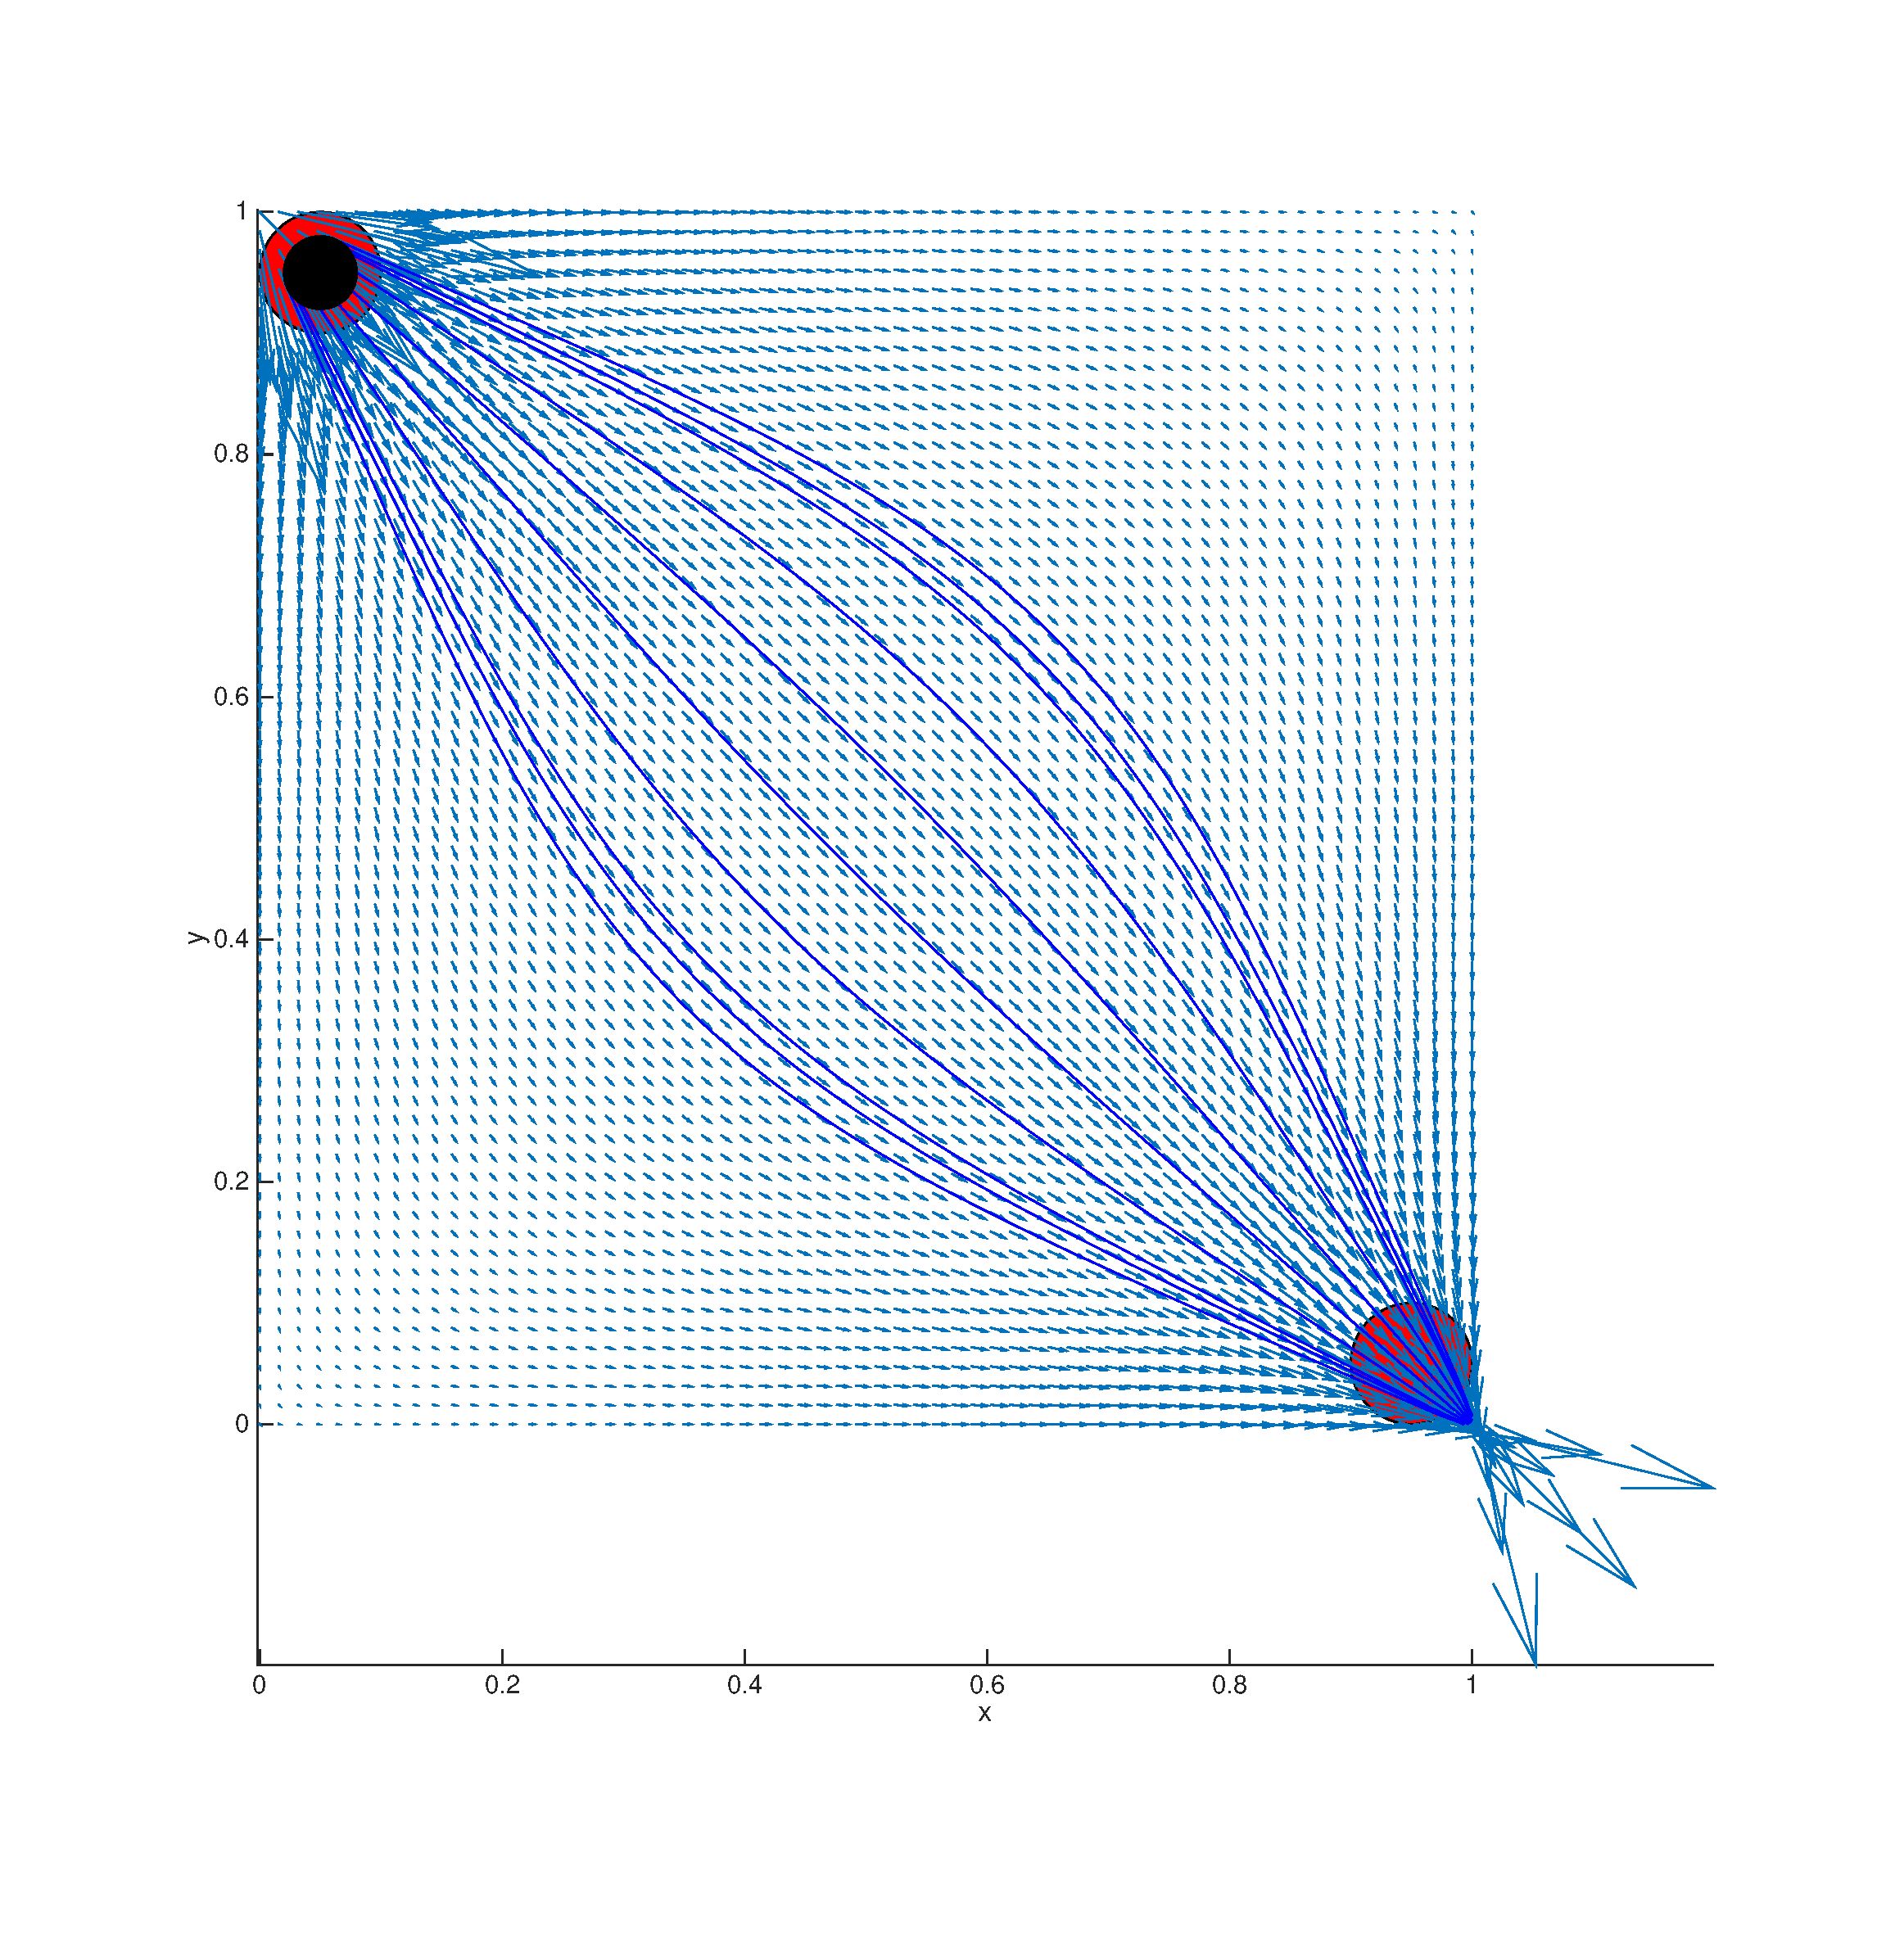
\includegraphics[width=15cm]{./figs/SourceSink.eps}
		\caption{Streamlines passing through the source. Source- and sink areas are shown in red. Streamlines are supposed to begin on $\partial B_\delta$ (black)}
		\label{fig:SourceSink}		
\end{figure}
Hence we conclude that if we know the solution on $\partial B_\delta$ we know the solution everywhere in $\Omega$. 

ODE \eqref{eq:ODEC}, which governs the behavior along the streamline, has the general solution
\begin{equation}\label{eq:Sol}
	c(s) = \int_{0}^{s} e^{-(R(s)-R(v))}c_a(v)\frac{\Qso(v)}{\phi(v)} \diff v.
\end{equation}
Here $R(v)=\int_{0}^v\Qso(x(u))/\phi(x(u)) d u$.
We can interpret $R(v)$ as the amount of contrast agent which is ,,accumulated'' while the particle moves through the source field.
Since in our setting $\Qso(x)=\qi$ for $x \in B_\epsilon$ and $\Qso(x)=0$ for $x \notin B_\epsilon$,  we find that $R(v)$ is constant if $v$ is bigger then some (streamline-dependent) threshold.
% We will now try to simplify \eqref{eq:Sol}. First, let us assume that $\phi(x) = \phi$ for some $\phi \in \R$, i.e. $\phi$ is a constant within $\Omega$. In this case we can solve \eqref{eq:ODEt} directly and obtain:
% \[
% 	t(s) = \phi s + t_0 \quad \Leftrightarrow \quad s = (t - t_0)/\phi
% \]
% where $t_0$ is the starting-timepoint of the particles we want to track.
% In order to go back to an Eulerian formulation, we can hence eliminate the parametrization variables $s$ and switch to a parametrization by regular time instead.
% Substituting $v = (w-t_0)/\phi$ and setting $t_0 + s\phi = t$ in \eqref{eq:Sol} yields:
% \begin{equation}
% 	\label{eq:Solt}
% 	c(t) = \frac{1}{\phi}\int_{t_0}^t e^{-\left(R(\frac{t-t_0}{\phi})-R(\frac{w-t_0}{\phi}\right)}c_a\big(\frac{w-t_0}{\phi}\big)\Qso\big(\frac{v-t_0}{\phi}\big) \frac{\diff w}{\phi}
% \end{equation}
% This equation can be interpreted as follows:
% For a given starting-point $x_0$ and starting time $t_0$, Eq. \eqref{eq:Solt} gives the concentration at timepoint $t$ and location $x((t-t_0)/\phi)$.
% Further assuming that $t$ is big enough that $x(t) \notin B_\epsilon$, we obtain $R(\frac{t-t_0}{\phi}) = \qi \cdot l$ for $l = (t_{max}-t_0)/\phi$ and $t_{max}$ is the timepoint at which $x(t)$ leaves the source-area $B_\epsilon$.
% \CHalert{I am still working on the following section:}
% This yields the following expression for $c(t)$:
% \[
% 	c(t) =
% \]
% We will now try to go back to an Eulerian Formulation: One can see that for constant $k:=(t-t_0)/\phi$ we have also a constant location $x_k:=x(k)$.
% This gives the following concentration at location $x_k$ in dependency of the starting-time $t_0$:
% \[
% 	c(x_k,t_0 + k \phi) = \frac{1}{\phi}\int_{t_0}^{t_0 + k\phi} e^{-\left(R(t)-R(\frac{w-t_0}{\phi}\right)}c_a\big(\frac{w-t_0}{\phi}\big)\Qso\big(\frac{v-t_0}{\phi}\big) \frac{\diff w}{\phi}
% \]
% Since no tracer will arrive before timepoint $0+\phi k$ at $x_k$, we get the following closed expression for
% \CHalert{BEGIN COMMENT HERE, ONLY FOR OUR UNDERSTANDING}
% \\
% \begin{equation}
% c(x_0,t) = e^{-R(t)}\Big (\int_{0}^t e^{R(s)} F(x_0,s)ds\Big )
% \end{equation}
%  This is again equivalent with
% \begin{equation}
% c(x_0,t) = \int_{0}^t e^{-(R(t) - R(s))} F(x_0,s)ds
% \end{equation}
% and inserting the expression for $F$ leads to
% \begin{equation}
% c(x_0,t) = \frac{Q_{so}(x_0)}{\phi(x_0)} \int_{0}^t e^{-(R(t) - R(s))}c_{so}(x_0,s) ds
% \end{equation}
% \\
% END BEGIN COMMENT HERE
% \\
Backpropagating $C = c \phi$ and inserting the expression for $F$ results in
\begin{equation}
C(x_0,t) = Q_{so}(x_0) \int_{0}^t e^{-(t - s)/T}c_{so}(x_0,s) ds
\label{eq:Cpdeclassic}
\end{equation}
for the mean transit time $T := \phi(x_0) / Q_{so}(x_0)$.
A comparison with (\ref{eq:Cconv}) shows that these expressions are equal provided $P \rightarrow Q_{so}$ and $c_{so} \rightarrow c_{a}$. Thus, we have shown that the classical model is equivalent to a field model for tracer transport for specific requirements of the perfusion $P$ and the arterial input concentration $c_a$. (i) The first observation is that the computed perfusion $P$ is the actual flow at the inlet of the entire domain $\Omega$, and not the inlet of a further spatial sub-division. (ii) The second observation is the fact that the arterial input concentration $c_a$ is identical to the concentration at the source of $\Omega$. This is unproblematic since it is in agreement with the understanding of $c_a$. However, the first observation regarding the perfusion implies that the computed perfusion along the streamlines will be constant for various $t$ due to stationarity, and hence, computing the voxel wise perfusion for all voxels lying on the streamlines will over-estimate the perfusion with a factor varying with the streamline length. From this argument, we can predict that applying the classical model voxel wise will over-estimate the total perfusion within an arbitrary domain $\Omega$.

Integrating over $\Omega$ on both sides of (\ref{eq:Cpdeclassic}), and defining the average concentration $\overline{C}(t):= \frac{1}{|\Omega|}\int_{\Omega}C(x_0,t)dx$, 
\begin{equation}
\overline{C}(t) = \frac{1}{|\Omega|}\int_{\Omega} Q_{so}(x_0)  \int_{0}^t e^{-(t - s)/T}c_{so}(x_0,s) ds dx
\label{eq:Cpdeclassicroi}
\end{equation}
Since $Q_{so}(x_0)$ is only nonzero across $B_\epsilon$ we can write
\begin{equation}
\overline{C}(t) = \frac{1}{|\Omega|}\int_{B_\epsilon} Q_{so}(x_0)  \int_{0}^t e^{-(t - s)/T}c_{so}(x_0,s) ds dx
\label{eq:Cpdeclassicroitemp}
\end{equation}
For a constant source flow $\tilde{Q}_{so}$ within $B_\epsilon$, $\tilde{Q}_{so} = Q(x_0), x_0 \in B_\epsilon$, this is equivalent to
\begin{equation}
\overline{C}(t) = \frac{\tilde{Q}_{so}}{|\Omega|}\int_{B_\epsilon}  \int_{0}^t e^{-(t - s)/T}c_{so}(x_0,s) ds dx
\label{eq:Cpdeclassicroitemp}
\end{equation}
Further, for a content arterial input concentration $\tilde{c}_{so}(t)$ across $B_\epsilon$, $\tilde{c}_{so}(t) := c(x_0,t), x_0 \in B_\epsilon$ we can write
\begin{equation}
\overline{C}(t) = \frac{\tilde{Q}_{so} |B_\epsilon|}{|\Omega|}  \int_{0}^t e^{-(t - s)/T}\overline{c}_{so}(s) ds
\label{eq:Cpdeclassicroitemp}
\end{equation}
This is recognized as the total perfusion $P = \overline{Q}_{so}|B_\epsilon|/|\Omega|$, which is the total source flow divided by the total distributing domain $|\Omega|$. Hence, we can state that the averaging PDE model is consistent with
\begin{equation}
\overline{C}(t) = P \int_{0}^t e^{-(t - s)/T}\overline{c}_{so}(s) ds,
\label{eq:Cpdeclassicroitemp}
\end{equation}
This expression is identical to the classical model in (\ref{eq:Cconv}) for $\Omega$ as the averaging domain and by taking $c_{so}(t) = c_a(t)$.

Thus, we have in this section formally proven that the classical model for perfusion is correct when applying $\Omega$ as the averaging domain. On the other hand, applying the same model voxel wise will lead to an over-estimation of the perfusion, with a scaling factor growing along with the streamline length.

\subsection{A PDE-Model for the impuls-response functions}
		In order to understand the model better, we will derive in this section an equation for the impuls-response functions associated with a solution of \eqref{eq:conteqlocal}.
		Let us assume that there exists a solution and that the solution can be represented in the following way:
		\[
			c(x,t) = \int_0^t c_a(s)I(x,t-s)\diff s.
		\]
		We will now use this relationship together with \eqref{eq:conteqlocal}.
		In order to do that, we calculate the derivative with respect to $t$.
		This is done as follows:
		\begin{alignat*}{2}
			\frac{\diff}{\diff t} \int_0^t c_a(s)I(x,t-s)\diff s &= \lim_{h \to 0} \quad & &\frac{\int_0^{t+h} c_a(s)I(x,t+h-s)\diff s - \int_0^{t} c_a(s)I(x,t-s)\diff s}{h} \\
			&= \lim_{h \to 0} &&\frac{\int_0^{t} c_a(s)\left(I(x,t+h-s)-I(x,t-s) \right)\diff s}{h} \\
				&&&+ \frac{1}{h}\int_t^{t+h} c_a(s)I(x,t+h-s)\diff s. \\
				&= &&\int_0^t c_a(s) I_t(x,t-s) \diff s + c_a(t)I(x,0).
		\end{alignat*}
		Assuming that $I(x,0)=0$ \CHalert{(from the looks of the impuls-response functions obtained from the data this should hold)}, we obtain:
		\[
			\frac{\diff}{\diff t} \int_0^t c_a(s)I(x,t-s)\diff s = \int_0^t c_a(s)I_t(x,t-s)\diff s.
		\]
		Combining this with \eqref{eq:conteqlocal} yields:
		\begin{align*}
			\int_0^t c_a(s) &\big[ \phi I_t(x,t-s) + \nabla \cdot \left(\q(x)  I(x,t-s) \right) \\ 
			&+ I(x,t-s)\Qsi(x) -  \delta_0(t-s)\Qso(x) \big]  \diff s = 0.
		\end{align*}
		where $\delta_0$ is the delta-distribution with respect to time.
		Let us denote the term in squared brackets with $J(x,t)$, then we can write this equation as
		\[
			\int_0^t c_a(s) J(x,t-s) \diff s = 0 \quad \text{for all }x \in \Omega.
		\]
		The following lemma shows that this implies that $J(x,t) = 0$ for all $x \in \Omega, t \in [0,\infty)$.
		We analyze the above equation for an arbitrary point in $\Omega$.
		\begin{lemma}
			Let $j,c_a:[0,\infty) \to \R$ be continuous and assume that $c_a \not\equiv 0$. If it holds for all $t>0$ that
			\[
				\int_0^t c_a(s) j(t-s) \diff s = 0
			\]
			then $j\equiv 0$.
		\end{lemma}
		\begin{proof}
			Assume that $j \neq 0$ and let $t_j$ be the largest $t \in [0,\infty)$ such that $j(t_j)=0$.
			Since we assumed that $j$ is continuous, there is a small interval $(t_j,t_j+\beta)$ where either $j>0$ or $j<0$.
			For sake of simplicity assume that $j>0$ on $(t_j,t_j+\beta)$, the case that $j(t_j)<0$ will follow analogously.
			For $c_a$ we analogously define the timepoint $t_c$ and analogously assume that $c_a>0$ on $(t_c, t_c + \delta)$.
			Let $\gamma:=\min(\alpha,\delta)$.
			Then it holds for $t_0 := t_c + t_j + \gamma$ that
			\[
				\int_0^{t_0} c_a(s) j(t-s) \diff s = \int_{t_0-\gamma}^{t_0} c_a(s)j(t-s) > 0.
			\]
			We can hence conclude the assertion.
		\end{proof}
		
		Next we observe that in our case $\Qso$ and $\Qsi$ are both independent of time.
		As a consequence, one can see that if $C$ has the above structure, $I(x,t)$ needs to fulfill the following equation:
		\[
			\phi I_t(x,t) - \nabla \cdot (\q(x)I(x,t)) = \delta_t\Qso(x) - I(x,t)\Qsi(x)
		\]
		Hence $I(x,t)$ can be regarded as a solution of a the transport equation with a Dirac-Delta as Arterial Input.



\section{Numerical implementation}

\subsection{Discretization of the single phase flow model}
\label{sec:flowmodel}
As a discretizastion scheme for the SF model we apply the two-point fixed approximation (TPFA) finite volume method. This scheme is based on conservation of physical quantities across cell volumes. Denote a grid cell (voxel) as $\Omega_i$ and apply to (\ref{eq:flowmodel}) an integral over $\Omega_i$
\begin{equation}
\int_{\Omega_i} \nabla \cdot \Big ( -\frac{K}{\mu} \nabla p\Big )dx = \int_{\Omega_i}Qdx.
\end{equation}
This can in terms of the divergence theorem be rewritten as
\begin{equation}
\int_{\partial \Omega_i}   -(\lambda \nabla p) \cdot \nu ds = \int_{\Omega_i}Qdx = F_i.
\label{eq:TPFAint}
\end{equation}
for the conductivities $\lambda = K/\mu$. The integrated source term is per definition named as $F_i$ and has units of absolute flow, $m^3/s$. Let $\gamma_{ij}= \partial \Omega_i \cap \partial \Omega_j$ be the adjacent face between voxel $i$ and voxel $j$. Only the component of the pressure gradient perpendicular to $\gamma_{ij}$ will drive the flow between voxel $i$ and $j$. The component of $\nabla p$ pointing along the normal vector of $\gamma_{ij}$ can therefore be replaced in terms of the cell centred pressure values $p_i$ and $p_j$
\begin{equation}
\delta p_{ij} = \frac{2(p_j - p_i)}{\Delta x_i + \Delta x_j}
\end{equation}
where $\Delta x_{i}$ and $\Delta x_{j}$ are the cell dimensions in the respective grid direction for voxel $i$ and $j$, respectively.
The total flux $v_{ij}$ across the face $\gamma_{ij}$, the left hand side of (\ref{eq:TPFAint}), is thereby approximated by
\begin{equation}
v_{ij} = \delta p_{ij}\int_{\gamma_{ij}}\lambda ds.
\end{equation}
The conductivies $\lambda$ are defined at the cell centers, and must be approximated on the faces where the flux is measured. This can be achieved by a distance-weighted harmonic averaging. Let $\lambda_{i,ij} = n_{ij}\cdot \lambda_i n_{ij}$ and $\lambda_{j,ij} = n_{ji}\cdot \lambda_j n_{ij}$ and the directional permeability along $n_{ij}$ is computed as 
\begin{equation}
\lambda_{ij} = (\Delta x_i + \Delta x_j)\Big ( \frac{\Delta x_i}{\lambda_{i,ij}} + \frac{\Delta x_j}{\lambda_{j,ij}}\Big )^{-1}.
\end{equation}
Thus, for an orthogonal grid along the main coordinate axes we can approximate the flux across $\gamma_{ij}$ as 
\begin{equation}
v_{ij} = -|\gamma_{ij}|\lambda_{ij}\delta p_{ij} = 2|\gamma_{ij}|\Big ( \frac{\Delta x_i}{\lambda_{i,ij}} + \frac{\Delta x_j}{\lambda_{j,ij}}\Big )^{-1}(p_i - p_j)
\end{equation}
where $|\gamma_{ij}|$ is notation for the surface area of $\gamma_{ij}$.
The terms not depending on the pressure $p$ can be collected into the transmissibilities $t_{ij}$
\begin{equation}
t_{ij} =  2|\gamma_{ij}|\Big ( \frac{\Delta x_i}{\lambda_{i,ij}} + \frac{\Delta x_j}{\lambda_{j,ij}}\Big )^{-1}.
\end{equation}
From equation (\ref{eq:TPFAint}), summing over all faces $\gamma_{ij}$ surrounding voxel $i$, $j \in \mathbb{N}_i$ for the set of neighbour indices $\mathbb{N}_i$ at voxel $i$, results in a linear equation in the unknowns $p_i$ and $p_j$
\begin{equation}
\sum_{j \in \mathbb{N}_i}t_{ij}(p_i - p_j) = F_i ~~~ \forall \mbox{    }  \Omega_{i} \subset \Omega
\label{eq:TPFAlin}
\end{equation}
for each voxel.  Denote by $n = n_xn_yn_z$ the total number of voxels within $\Omega$. The left hand side term in (\ref{eq:TPFAlin}) yields a band diagonal matrix $A$ for the transmissibilities. Solving the linear system in (\ref{eq:TPFAlin}) provides the cell centered voxel wise values of the pressure $p_i$.
Note that the flux is discretized on a staggered grid, corresponding to the voxel faces, whereas the pressure, porosity and permeability are all discretized on a cell-centered grid, as shown in Fig. \ref{fig:grid}. Thus, the obtained flux field from applying (\ref{eq:syntdarcysimp}) is descretized on a staggered grid, along with the transmissibilities.
\begin{figure}[H]
	\centering
		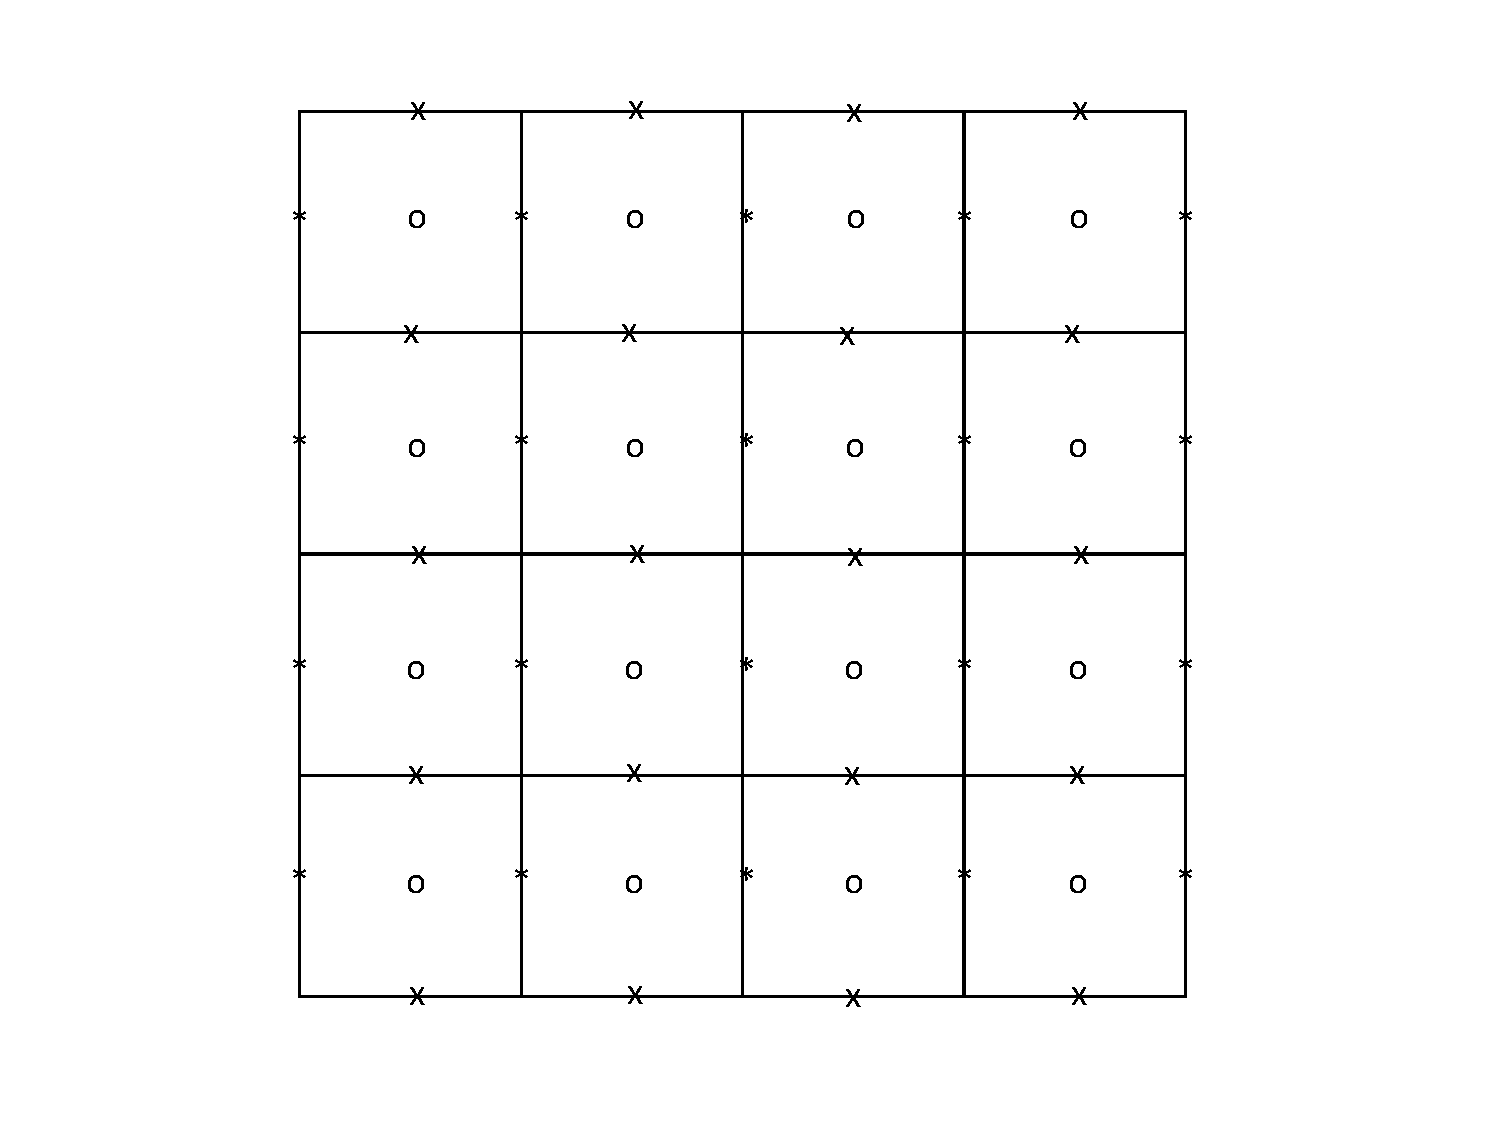
\includegraphics[width=0.7\textwidth]{figs/flowgrid.pdf}
	\caption{Grid for discretisation of the flow model in (\ref{eq:syntdarcysimp}) and (\ref{eq:flowmodel}). The circles represent cell centers where the pressure, porosity and permeability are defined. The "$\times$" and the "*" are staggered grid representations for discretisation of the flux in the vertical and horizontal direction, respectively.}
	\label{fig:grid}
\end{figure}



\subsection{Discretization of the indicator dilution flow model}


Let $c_i$ be the center voxel tracer concentration and $c_j$ the neighbour voxel concentration which the common face $\gamma_{ij}$. Consider Eq. (\ref{eq:conteq2}) for averaged quantities across cell volumes and faces,
\begin{equation}
	\phi_i V_i \frac{c_i^{t+1} - c_i^t}{\Delta t}  = - \sum_{j = 1}^{nf}c^t_{E_{j}}q_{\gamma_{ij}}|\gamma_{ij}| + c^t_{so,i}F_{so,i} + c^t_iF_{si,i}
	\label{eq:discsyntflowtracer}
\end{equation}
where the understanding of $q_{\gamma_{ij}}$ is the normal flux across face $\gamma_{ij}$, $c_{\gamma_{ij}}^t$ is the tracer concentration at face $\gamma_{ij}$ and $c_{so,i}^t$ is the tracer concentration of the source fluid entering the system (the AIF). The terms $F_{so,i} = Q_{so,i}V_i$ and $F_{si,i} = Q_{si,i}V_i$. However, the tracer concentrations are not discretized at the faces but rather at the cell centres, and we must apply an upwinding Godunov scheme for a proper representation. Let
\begin{equation*}
c^t_{E_j} = \left\{
\begin{array}{rl}
c^t_i & \text{if } q_{\gamma_{ij}} > 0, \text{   outward flux}\\
c^t_j & \text{if } q_{\gamma_{ij}} < 0, \text{   inward flux.}
\end{array} \right.
\end{equation*}
From (\ref{eq:discsyntflowtracer}), this leads to the explicit forward scheme
\begin{equation}
c_i^{t+1} = c_i^t + \frac{\Delta t}{\phi_i V_i}\Big [(c_{so,i}^tF_{so,i} + c_i^t F_{si,i})-\sum_{j = 1}^{nf}c_{E_j}^tq_{\gamma_{ij}}|\gamma_{ij}|\Big ]
\label{eq:forwdiscr}
\end{equation}
for each voxel $i$.
A conversion of $c_i$ into $C_i$ is performed via the relation $C_i = c_i\phi_i$. The overall concentration map $C_i$ is later used for the inverse problem of restoring CBV and CBF. 

\subsection{Estimating the streamline length}
\label{sec:streamline}
The streamline length $|\mathbb{C}|$ was computed according to
$$
	r_{i+1} = r_i + \epsilon q(r_i), 	~~ i = 0,1,\hdots
$$
for a small step length $\epsilon = 0.3$ and the parameterised streamline $r$.
Initiating the integration from the source or sink was not possible since the streamlines then are diverging. Instead, we computed a continuous line of equidistant voxels from the source and the sink and initiated the integration in both directions from these positions. Thus, we would instead follow the vector field as it is joining instead of diverging. The length of the streamlines was assigned as the total integration length in both directions towards the source and the sink from the line of equidistant voxels as initial positions $r_0$. Due to discretization errors, increasingly multiple assignments of stream line length will take place as approaching the source and sink. For these voxels we assign the minimum length for every voxel. 



\section{Numerical experiments}

\subsection{Simulations on the single phase flow field}

A table of parameter values used for the numeral simulations are shown in Table \ref{tab:par}. We aimed at creating a transparent synthetic test case and kept all optional parameters as simple as possible. Therefore, the permeability and porosity were constant valued in space.
\begin{table}[H]
\centering
  \begin{tabular}{ l | c | c | r }
  Description & Symbol & Value(s) & Unit \\
  \hline
    	Average input perfusion & $\overline{P}$ & $50$ & $ml/min/100ml$  \\
	Flow source, derived from $\overline{P}$ & $F_{so}$ & $0.08333$ & $mm^3/s$  \\
	Flow sink & $F_{si}$ & $-F_{so}$ & $mm^3/s$  \\
	Dynamic viscosity blood \cite{Rosencranz2006} & $\mu_b$ & $5 \cdot 10^{-6}$ & $kPa\cdot s$  \\
	Fluid density blood \cite{Kenner1989} & $\rho$ &  $1 $ & $mg/mm^3$ \\		
	Permeability  & $k$ &  $5 \cdot 10^{-6}$ & $mm^2$ \\	
	Porosity & $\phi$ &  $0.05$ &  $mm^3/mm^3$\\	
	Spatial resolution & $R$ & $(64,64,1)$ & -\\
	Physical dimension & $D$ & $(10,10,1)$ & $mm$\\
	Voxel size & $h$ & $(0.156,0.156,1)$ & $mm$\\
  \end{tabular}
  \caption{Parameters used in the numerical experiments, optimized for a slab of the capillary system in the human brain. For the viscosity of non-Newtonian blood we used a suitable setting of dynamic viscosity. The scalar permeability $k$ was added to the diagonal terms of $K$, such that $K_{ii} = k$  for $ i = \{1,2 \}$. The porosity had a fixed value everywhere (cite paper Constantin).}
  \label{tab:par}
\end{table}
Results from the discretized flow model described in (\ref{eq:TPFAlin}) are shown in Fig. \ref{fig:flowsyntresults} for the pressure field $p$, the flux vector field $q$ and the perfusion $P$. The pressure field can only be estimated up to a constant and was therefore scaled such that the minimum value is always zero. We used average input perfusion values of $\overline{P} = 50ml/min/100ml$, targeted towards the human brain. For the specified physical dimension $D$ we computed the flow source from the average input perfusion by multiplying with the physical volume $D$ and converting to $mm$ and $s$ as units for space and time. 
The computed perfusion field $P$ had an average value of $50.5ml/min/100ml$, which is close to the average input perfusion $\overline{P}$ used to compute the source flow $F_{so}$.



The source term was chosen to the upper left voxel and the sink term was chosen in the lower right voxel. The inflow in the source was set negatively to the outflow in the sink, $F_{so} = -F_{si}$. Note that the source term is only nonzero within the domain of the source, and similar for the sink
\begin{equation*}
F_i(x) =
\begin{cases}
F_{so} & \text{if } x_i \in \Omega_{so},\\
F_{si} & \text{if } x_i \in \Omega_{si},\\
0 & \text{elsewhere }
\end{cases}
\end{equation*}
for the source domain $\Omega_{so}$ and sink domain $\Omega_{si}$.


\begin{figure}[H]
        \centering
                \subfloat[Pressure field, $p$.]{
                \begin{overpic}[width=0.50\textwidth]{figs/synt-createflowTPFA-phi-flat-K-flat-dim-64-p.eps}
                \end{overpic} }
                \subfloat[Flux vertical direction, $q_1$.]{
                \begin{overpic}[width=0.50\textwidth]{figs/synt-createflowTPFA-phi-flat-K-flat-dim-64-fluxx.eps}
                \end{overpic} }\\
	       \subfloat[Flux horizontal direction, $q_2$.]{
                \begin{overpic}[width=0.50\textwidth]{figs/synt-createflowTPFA-phi-flat-K-flat-dim-64-fluxy.eps}
                \end{overpic}}
	       \subfloat[Perfusion $P$ according to (\ref{eq:flux2perf})]{
                \begin{overpic}[width=0.50\textwidth]{figs/synt-createflowTPFA-phi-flat-K-flat-dim-64-perfn.eps}
                \end{overpic}}
        \caption{Synthetic flow model with a source in the upper left corner and a sink in the lower right corner. (a) Pressure field from solving the linear system in (\ref{eq:TPFAlin}), (b-c) flux multiplied by voxel face area $q_1h_yh_z,q_2 h_xh_z$ $[mm^3/s]$ in vertical and horizontal direction with positive directions downward and right, respectively. (c) Voxelwise estimated perfusion $[ml/min/100ml]$ according to (\ref{eq:flux2perf}).}
        \label{fig:flowsyntresults}
\end{figure}
                                   
The voxelwise streamline length was computed from the flux field $q$ as described in section \ref{sec:streamline}. The streamline length for the flux field in Fig. \ref{fig:flowsyntresults} is shown in Fig. \ref{fig:streamlinelength}.
\begin{figure}[H]
	\centering
		\includegraphics[width=0.50\textwidth]{figs/synt-createflowTPFA-phi-flat-K-flat-dim-64-lenmat.eps}
	\caption{Length of streamlines $|\mathbb{C}|$ $(mm)$ of the flux field shown in Fig. \ref{fig:flowsyntresults}.}
	\label{fig:streamlinelength}
\end{figure}
The perfusion map in Fig. \ref{fig:flowsyntresults} was computed from Eq. (\ref{eq:flux2perf}) using the flux field shown in Fig. \ref{fig:flowsyntresults} and the length of streamlines shown in Fig. \ref{fig:streamlinelength}.

\subsection{The AIF input curve}
For the incoming arterial input function we applied two well established variants of the AIF, First, we model the AIF as an analytical gamma function according to [Wu, Ostergaard]. Second, we use the empirically averaged Parker AIF [Parker 2006]. These two AIF functions are shown in Fig. \ref{fig:AIF}.
\begin{figure}[H]
	\centering
		\includegraphics[width=0.50\textwidth]{figs/makefigs-AIF-phi-flat-K-flat-dim-64-aif-gamma-T-90.eps}
	\caption{The two AIF curves used for simulations. The Gamma AIF is an analytical function while the Parker AIF is an averaged response curve observed in real experiments.}
	\label{fig:AIF}
\end{figure}


\subsection{Simulations on the simulated flow model}
The SF model was implemented according to (\ref{eq:forwdiscr}) and the previously obtained flux field. The results are shown in Figs. \ref{fig:flowsynttracergamma} and \ref{fig:flowsynttracerparker} for the gamma and Parker AIF, respectively.
\begin{figure}[H]
	\centering
		\includegraphics[width=0.99\textwidth]{figs/synt-createindicatorpde-phi-flat-K-flat-dim-64-aif-gamma-T-90-panel.eps}
	\caption{Development of tracer $C(x,t)$ as a function of time using the gamma AIF. The plots show the tracer concentration for equidistant time points, from top to bottom and left to right of the panels. The entire simulation was run for $90s$ but only the first half of the simulation is plotted.}
	\label{fig:flowsynttracergamma}
\end{figure}
\begin{figure}[H]
	\centering
		\includegraphics[width=0.99\textwidth]{figs/synt-createindicatorpde-phi-flat-K-flat-dim-64-aif-parker-T-90-panel.eps}
	\caption{Development of tracer $C(x,t)$ as a function of time using the Parker AIF. The plots show the tracer concentration for equidistant time points, from top to bottom and left to right of the panels. The entire simulation was run for $90s$ but only the first half of the simulation is plotted.}
	\label{fig:flowsynttracerparker}
\end{figure}




\subsection{Experiments on the simulated convolution model}

In this section we present experimental data of the SC model Section \ref{sec:flowmodel}. We use realistic parameter values of the included parameters, as described in Table \ref{tab:par}, optimized for the human brain capillary system. We seek to model a small volume of the capillary system with physical dimension of $1cm \times 1cm \times 0.1 mm$. This corresponds to a 2D slab with thickness equal to $0.1mm$, and has a physically realistic extension in $x$ and $y$. All tissue parameters are constant in space.

Given the previously estimated voxelwise flow field from the PDE model we want simulate the flow field using (\ref{eq:Cconv1}). However, the classical theory does not take into account the timing of the arrival of the tracer, and the feeding of the indicator starts everywhere at the same time. Therefore we estimate a voxelwise delay field according to the maximum tracer concentrations within the synthetic field model. Denote this delay field as $\mu(x)$, and we get a slightly modified classical model
\begin{equation}
C(x,t) = P(x) \int_{0}^{t}e^{-\frac{t-s}{T}}c_A(s)ds
\label{eq:Cconv2}
\end{equation}
From now we also assume that the concentrations are now spatially dependent as $C = C(x,t)$, and similarly for the perfusion $P = P(x)$.
The delay field is essentially scaleable with a time-to-peak map and will not change the results of the forthcoming deconvolution but it generates a concentration map which is physically plausible.

Simulation results using the PDE derived flow field as well as the classical model (\ref{eq:Cconv2}) is shown in Figs. \ref{fig:flowsyntconvtracergamma} and \ref{fig:flowsyntconvtracerparker}. 

%\begin{figure}[H]
%	\centering
%		\includegraphics[width=0.99\textwidth]{figs/syntconv-createindicatorconv-phi-flat-K-flat-dim-64-aif-gamma-T-90-panel.eps}
%	\caption{Development of tracer $C(t)$ as a function of time using the synthetic convolution approach and the gamma AIF. The plots show the tracer concentration for equidistant time points from top to bottom and left to right of the panels. The entire simulation was run for $90s$.}
%	\label{fig:flowsyntconvtracergamma}
%\end{figure}
%
%\begin{figure}[H]
%	\centering
%		\includegraphics[width=0.99\textwidth]{figs/syntconv-createindicatorconv-phi-flat-K-flat-dim-64-aif-parker-T-90-panel.eps}
%	\caption{Development of tracer $C(t)$ as a function of time using the synthetic convolution approach and the Parker AIF. The plots show the tracer concentration for equidistant time points from top to bottom and left to right of the panels. The entire simulation was run for $90s$.}
%	\label{fig:flowsyntconvtracerparker}
%\end{figure}


\subsection{Comparing the SF and SC model in terms of concentration maps}

The percentage difference between the SF and the SC model was computed as
\begin{equation}
d_i = 100 \frac{\frac{1}{|\Omega|}\sum_{x_i \in \Omega} \big (C_{SF}(x_i,t_i) - C_{SC}(x_i,t_i)\big )}{\overline{C}_{SF}(x_i,t_i)}
\end{equation}
where $\overline{C}_{SF}(x_i)$ is the voxelwise average value of $C_{SF}$ across time. The average deviation $\overline{d}$ was $88.5\%$ and $31.2\%$ for the gamma and Parker AIF, respectively. These average tracer concentration is plotted over time in Fig. \ref{fig:compareindicator} and we see that the convolution partly fails to describe the flow field from the SF model.

\begin{figure}[H]
	\centering
		\includegraphics[width=0.50\textwidth]{figs/makefigs-compareindicator-phi-flat-K-flat-dim-64.eps}
	\caption{Average tracer concentration using the SF model and the SC model. Left: Gamma AIF. Right: Parker AIF.}
	\label{fig:compareindicator}
\end{figure}


\subsection{The maximum-slope model}
The maximum-slope model is the simplest model to recover perfusion.
We follow [?] in its the derivation.
Given a tissue-curve $C(t)$, an arterial input function $c_a(t)$ as well as a venous output function $c_v(t)$, it is assumed that for any given timepoint the following relationship is fulfilled:
\[
	C(t+\Delta t) - C(t) \approx P \cdot \Delta t \big(c_a(t) - c_v(t + \Delta t)\big).
\]
Here $\Delta t(c_a(t) - c_v(t + \Delta t))$ is the (approximate) total amount contrast-agent introduces in time $\Delta t$ and $C(t+\Delta t) - C(t)$ is the (approximate) amount of contrast agent which has been measured to pass through the system.
The Maximum-Slope model assumes that these two values are proportional with proportionality constant $P$, the perfusion. Rearranging and letting $\Delta t \to 0$ yields:
\[
	P = \frac{C'(t)}{c_a(t) - c_v(t)}.
\]
We now assume that we are in an early uptake-phase, where no contrast agent is leaving the system yet. 
Hence it holds approximately
\[
	P = \frac{C'(t)}{c_a(t)} \iff Pc_a(t) = C'(t).
\]
Differentiating this equation with respect to $t$ yields:
\[
	P c_a'(t) = C''(t).
\]
Since this equation is fulfilled for every timepoint $t$, it is fulfilled especially for timepoint $t_{\mathrm max}:=\mathrm{argmax}_{t}c_a(t)$. 
Since at this point it holds that $c_a'(t_{\mathrm max}) = 0$ and hence also $C''(t_{\mathrm max})=0$, we derive
\begin{equation}\label{eq:MS}
	P = \frac{\max_{t}C'(t)}{\max_{t}c_a(t)}.
\end{equation}


\section{Restoring the porosity and flow field using different models}

We tested the the convolution based classical model \eqref{eq:Cconv1} as well as maximum-slope model (MS, \eqref{eq:MS}) for their capability to recover the perfusion values.
The deconvolution was performed using the block circulant SVD (bSVD) approach described in [?], which comes with a time-invariance with respect to arrival times.
The success of the restoration was measured in terms of the relative error of the recovered perfusion with respect to the true perfusion
\[
	RE := \frac{\vert P_{\mathrm rec} - P_{\mathrm true}\vert}{P_{\mathrm true}}\cdot 100\%.
\]
The input data was downsampled to a final time-resolution of $\SI{1}{\second}$.
In order to simulate different spatial resolutions, the data was spatially averaged over different block-sizes ranging from $b_1 = (1,1)$ to $b_5=(64,64)$.
Results are displayed in Figure \ref{fig:resultsSCD},\ref{fig:resultsSFD} as well as in Table \ref{tab:resultsSim}.
It can be observed that for the complete domain the perfusion can be restored by both methods accurately with an error of $\approx 2\%$.
The impuls-response function reconstructed from the perfusion method is displayed in Figure \ref{fig:deconvResults}.
However, within the capillary field the model assumptions of one inlet and one outlet are violated, causing large errors in the recovered flow field.
Typical impuls response functions of the capillary field are also visualized in Figure \ref{fig:deconvResults}.
These recovered gaussian-like functions seem to be describing dispersion effects, yielding a smoothing and broadening of the arterial-input.


\begin{table}[H]
	\caption{Results of the perfusion restoration with median relative errors in percent. Relative error was computed block-wise as $\vert P_{\mathrm rec} - P_{\mathrm true}\vert / P_{\mathrm true}\cdot 100\%$. Displayed is the median RE over the entire domain.}
	\centering
		\begin{tabular}{l c c c c c }
			& Model & \multicolumn{4}{c}{Block Size}\\
			 					 			& 		& (1,1) 		& (5,5) 		& (10,10) 		& entire domain \\
			\toprule
			\multirow{2}{*}{SFD: Perfusion} & MS 	& $170.09$ 	& $165.03$ 	& $158.57$ 		& $2.65$ \\
			 					 	   		& bSVD  & $859.06$ 	& $768.58$ 	& $664.84$ 		& $1.25$ \\
			\multirow{2}{*}{SCD: Perfusion} & MS 	& $-23.20$ 	& $24.26$ 	& $25.75$ 		& $37.96$ \\
			 					 			& bSVD  & $2.43$ 		& $4.27$ 	& $8.80$ 	& $20.72$ \\
			\midrule											
			SFD: CBV & & $4.37\cdot10^{-5}$      & $4.37\cdot10^{-5}$		& $4.37\cdot10^{-5}$		& $4.37\cdot10^{-5}$ \\											
			SCD: CBV & & $1.94\cdot10^{-2}$      & $1.93\cdot10^{-2}$		& $2.12\cdot10^{-2}$		& $1.13$ 			
		\end{tabular}
	\label{tab:resultsSim}
\end{table}



\newcommand{\inc}[1]{\includegraphics[width = .3\textwidth]{./figs/#1}}
\newcommand{\rbox}[2]{\rotatebox{90}{\hspace{#1}\mbox{\large #2}}}
\begin{figure}[H]
	\caption{Results of the restoration of perfusion for the PDE Model (SFD) for different levels of discretization, displayed in the columns. All results are given in $\mathrm{ml/min/100ml}$. First Row: Ground-Truth Perfusion (cp. Sec. \ref{subsec:FluxToPerfusion}). Second Row: Perfusion as estimated by bSVD. Third Row: Perfusion as estimated by the Maximum-Slope model.}
	\centering
		\begin{tabular}{c c c c}
			 \rbox{5ex}{True perfusion} & \inc{recTrue-1.eps} & \inc{recTrue-5.eps} & \inc{recTrue-10.eps}\\
			 \rbox{13ex}{bSVD} & \inc{recCirc-pde-1.eps} & \inc{recCirc-pde-5.eps} & \inc{recCirc-pde-10.eps}\\
			 \rbox{13ex}{MS} & \inc{recMS-pde-1.eps} & \inc{recMS-pde-5.eps} & \inc{recMS-pde-10.eps}\\			 			 			  Block-Size & (1,1) & (5,5) & (10,10)
		\end{tabular}
	\label{fig:resultsSFD}
\end{figure}


\begin{figure}[H]
	\caption{Results of the restoration of perfusion for the Convolution Model (SCD) for different levels of discretization, displayed in the columns. All results are given in $\mathrm{ml/min/100ml}$. First Row: Ground-Truth Perfusion (cp. Sec. \ref{subsec:FluxToPerfusion}). Second Row: Perfusion as estimated by bSVD. Third Row: Perfusion as estimated by the Maximum-Slope model.}
	\centering
		\begin{tabular}{c c c c}
			 \rbox{5ex}{True perfusion} & \inc{recTrue-1.eps} & \inc{recTrue-5.eps} & \inc{recTrue-10.eps}\\
			 \rbox{13ex}{bSVD} & \inc{recCirc-conv-1.eps} & \inc{recCirc-conv-5.eps} & \inc{recCirc-conv-10.eps}\\
			 \rbox{13ex}{MS} & \inc{recMS-conv-1.eps} & \inc{recMS-conv-5.eps} & \inc{recMS-conv-10.eps}\\			 			 			  Block-Size & (1,1) & (5,5) & (10,10)			
		\end{tabular}
	\label{fig:resultsSCD}
\end{figure}



\begin{figure}[H]
	\caption{Results for the deconvolution model. First row: Results of bSVD applied to SFD with block-size (64,64) (i.e. entire domain) (Model-Fit and Impuls-Response Function). Second row: Results of bSVD applied to a single voxel of the SFD in the inside of the domain. Third row: Second row: Results of bSVD applied to a single voxel of the SCD in the inside of the domain.}
	\centering
		\begin{tabular}{c c c}
			 \rbox{0ex}{Entire Domain, SFD} & \inc{C-and-Crec.eps} & \inc{Irec.eps} \\
			 \rbox{2ex}{Inside the capillary bed, SFD}& \inc{C-and-Capprox-cap.eps} & \inc{IR-cap.eps} \\			 
			 \rbox{2ex}{Inside the capillary bed, SCD}& \inc{C-and-Crec-conv.eps} & \inc{Irec-conv.eps}			 
		\end{tabular}
	\label{fig:deconvResults}
\end{figure}



%
%
% For restoration of the perfusion flow field we apply a voxelwise deconvolution of (\ref{eq:Cconv2}). For deconvolution we used the regularized Levenberg-Marquardt least squares method (here referred to as method 'least-squares deconvolution') to solve the linear system $AR = C$, corresponding to a Tikhonov regularization with $\epsilon = 10^{-4}$. Additionally, we applied a circular SVD deconvolution which is considered the state-of-the-art method for deconvolution within perfusion applications (here referred to as the method 'circular SVD'). The results for reconstructed voxelwise perfusion and porosity are presented as percentage error
% $$
% \Delta P(\%) = \frac{P_{rec}-P}{P}100\%, ~~ \Delta \phi(\%) = \frac{\phi_{rec}-\phi}{\phi}100\%
% $$
% where $P_{rec}$ is the reconstructed perfusion and $\phi_{rec}$ is the reconstructed porosity.
% The reconstructions using a downsampling corresponding to a time spacing of $\Delta t = 0.2s$ is shown in Figs. \ref{fig:flowreconresultsgamma} - \ref{fig:flowreconresultsparker}.
%
% \begin{figure}[H]
%         \centering
% 	       \subfloat[$\Delta P$ for $\Delta t = 0.2s$.]{
%                 \begin{overpic}[width=0.45\textwidth]{figs/synt-reconflow-method-classic-phi-flat-K-flat-dim-64-aif-gamma-T-60-dcmethod-circSVD-red-100-perfn.eps}
%                 \end{overpic}}
% 	       \subfloat[$\Delta \phi$ for $\Delta t = 0.2s$.]{
%                 \begin{overpic}[width=0.45\textwidth]{figs/synt-reconflow-method-classic-phi-flat-K-flat-dim-64-aif-gamma-T-60-dcmethod-circSVD-red-100-porosity.eps}
%                 \end{overpic}}
%                 \\
% 	       \subfloat[$\Delta P$ for $\Delta t = 1s$.]{
%                 \begin{overpic}[width=0.45\textwidth]{figs/synt-reconflow-method-classic-phi-flat-K-flat-dim-64-aif-gamma-T-60-dcmethod-circSVD-red-500-perfn.eps}
%                 \end{overpic}}
% 	       \subfloat[$\Delta \phi$ for $\Delta t = 1s$.]{
%                 \begin{overpic}[width=0.45\textwidth]{figs/synt-reconflow-method-classic-phi-flat-K-flat-dim-64-aif-gamma-T-60-dcmethod-circSVD-red-500-porosity.eps}
%                 \end{overpic}}
%         \caption{Percentage error of reconstructed perfusion and porosity maps using the gamma AIF, SCD and for different time spacing. (a-b) $\Delta P(\%)$ and $\Delta \phi(\%)$ for $\Delta t = 0.2s$ (c-d) $\Delta P(\%)$ and $\Delta \phi(\%)$ for $\Delta t = 1s$. }
%         \label{fig:flowreconresultsgamma}
% \end{figure}
%
%
% \begin{figure}[H]
%         \centering
% 	       \subfloat[$\Delta P$ for $\Delta t = 0.2s$.]{
%                 \begin{overpic}[width=0.45\textwidth]{figs/synt-reconflow-method-classic-phi-flat-K-flat-dim-64-aif-parker-T-60-dcmethod-circSVD-red-100-perfn.eps}
%                 \end{overpic}}
% 	       \subfloat[$\Delta \phi$ for $\Delta t = 0.2s$.]{
%                 \begin{overpic}[width=0.45\textwidth]{figs/synt-reconflow-method-classic-phi-flat-K-flat-dim-64-aif-parker-T-60-dcmethod-circSVD-red-100-porosity.eps}
%                 \end{overpic}}
%                 \\
% 	       \subfloat[$\Delta P$ for $\Delta t = 1s$.]{
%                 \begin{overpic}[width=0.45\textwidth]{figs/synt-reconflow-method-classic-phi-flat-K-flat-dim-64-aif-parker-T-60-dcmethod-circSVD-red-500-perfn.eps}
%                 \end{overpic}}
% 	       \subfloat[$\Delta \phi$ for $\Delta t = 1s$.]{
%                 \begin{overpic}[width=0.45\textwidth]{figs/synt-reconflow-method-classic-phi-flat-K-flat-dim-64-aif-parker-T-60-dcmethod-circSVD-red-500-porosity.eps}
%                 \end{overpic}}
%         \caption{Percentage error of reconstructed perfusion and porosity maps using the Parker AIF, SCD and for different time spacing. (a-b) $\Delta P(\%)$ and $\Delta \phi(\%)$ for $\Delta t = 0.2s$ (c-d) $\Delta P(\%)$ and $\Delta \phi(\%)$ for $\Delta t = 1s$. }
%         \label{fig:flowreconresultsparker}
% \end{figure}
%
%
%
% \begin{table}[H]
% \scriptsize
% \begin{center}
% \begin{tabular}{ l  l  l  l  l  l  l  l  l }
%  & parker-ls-0.2s & parker-ls-1s & parker-circSVD-0.2s & parker-circSVD-1s & gamma-ls-0.2s & gamma-ls-1s & gamma-circSVD-0.2s & gamma-circSVD-1s\\
% \hline
% Perfusion, SFD &  61.16 &  61.22 & 5299.63 & 773.21 &  66.06 &  66.22 & 815.54 & 489.96\\
% Porosity, SFD &   3.19 &   3.19 &   3.19 &   3.19 &   0.00 &   0.02 &   0.00 &   0.02\\
% Perfusion, SCD &  74.66 &  73.34 & 5644.59 & 812.18 &  85.23 &  84.43 & 76761.61 &   1.17\\
% Porosity, SCD &  13.06 &  12.83 &  13.06 &  12.83 &   4.31 &  10.83 &   4.31 &  10.83\\
% \hline
% \end{tabular}
% \end{center}
% \caption{Average percentage error to the true perfusion and porosity fields, computed as $\overline{|\Delta P |}$ and $\overline{|\Delta \phi |}$. SFD= Simulated flow data from Darcys law and indicator-dilution theory. SCD = Simulated convolution data. The porosity has generally very low errors, although the error is higher for the Parker AIF than for the gamma AIF.  'ls' = least squares deconvolution and 'circSVD' = circular SVD deconvolution. The deviations for the perfusion are generally large.}
% \label{tab:results}
% \end{table}


\bibliographystyle{plain} 
%\bibliography{erlend}
%\bibliography{/home/erlend/disk/5/latex/erlend}
\bibliography{/Users/erlend/Documents/prosjekter/latex/erlend}



% that's all folks
\end{document}










